%Made By Thomas Debelle
\documentclass{report}
\usepackage[a4paper, total={6in, 9in}]{geometry}
\usepackage[utf8]{inputenc}
\usepackage[french]{babel}
\usepackage{graphicx}
\usepackage{graphics}
\usepackage[T1]{fontenc}
\usepackage{amsmath}
\usepackage{hyperref}
\usepackage{amssymb}
\usepackage{listings}
\usepackage{xcolor}
\usepackage{array}
\usepackage{float}
\usepackage{amsfonts}
\usepackage{fancyhdr}
\usepackage{titlesec}
\usepackage{xparse}
\usepackage{wrapfig}
\usepackage{enumitem}

\hypersetup{
    colorlinks=true,
    linkcolor=black,
    filecolor=magenta,
    urlcolor=cyan,
    pdftitle={Overleaf Example},
    pdfpagemode=FullScreen,
    }
\begin{document}


\begin{titlepage}
    \begin{figure}
        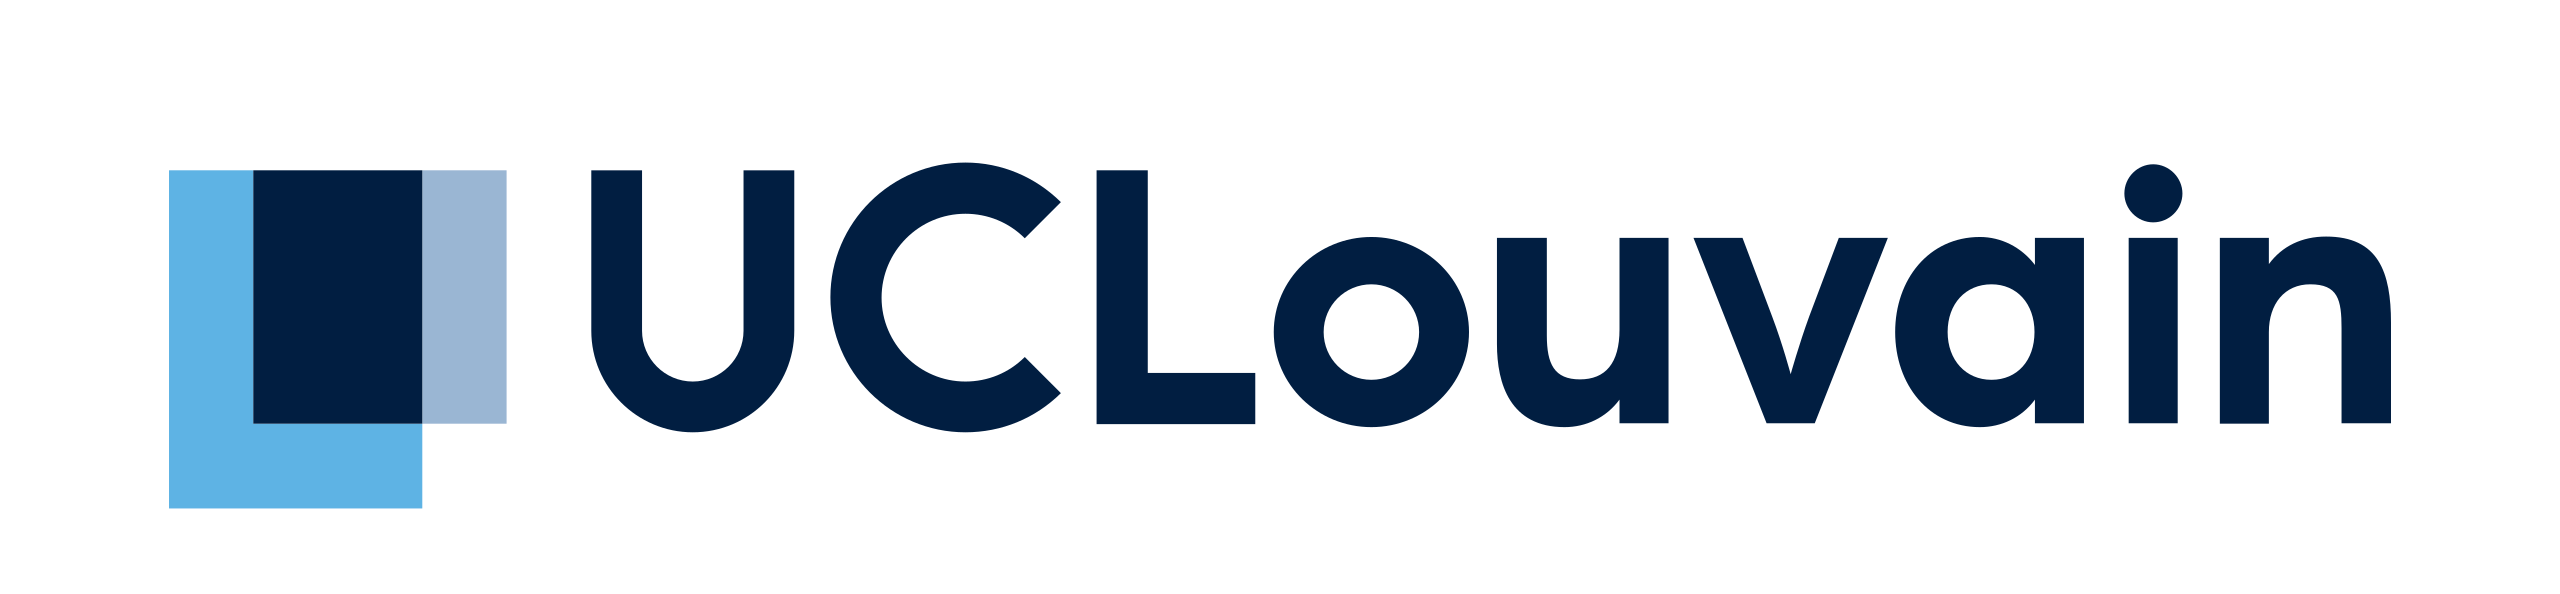
\includegraphics[height = 2cm]{UCL_Logo.png}
        \label{fig:my_label}
    \end{figure}

    \hspace*{100cm}
    \centering
    \vspace*{7cm}

    {\Huge \textbf{Résumé de LELEC1370}}\\
    \vspace*{0.25cm}
    compilation du \today\\
    \vspace*{0.25cm}
    \Large{Thomas Debelle}\\

    \vspace*{9.5cm}
    {\Large Juin 2023}
\end{titlepage}


\tableofcontents
\newpage

\section*{Préface}

Bonjour à toi !\\

Cette synthèse recueille toutes les informations importantes données au cours, pendant les séances de tp et est améliorée grâce au note du Syllabus. Elle ne remplace pas le cours donc écoutez bien les conseils et potentielles astuces que les professeurs peuvent vous donner. Notre synthèse est plus une aide qui, on l'espère, vous sera à toutes et tous utile.\\

Elle a été réalisée par toutes les personnes que tu vois mentionnées. Si jamais cette synthèse a une faute, manque de précision, typo ou n'est pas à jour par rapport à la matière actuelle ou bien que tu veux simplement contribuer en y apportant tes connaissances ? Rien de plus simple ! Améliore la en te rendant \href{http://www.github.com/Tfloow/Q4_EPL}{ici} où tu trouveras toutes les infos pour mettre ce document à jour. (\textit{en plus tu auras ton nom en gros ici et sur la page du github})\\

Nous espérons que cette synthèse te sera utile d'une quelconque manière ! Bonne lecture et bonne étude.


\chapter{Cours 1}
\section{Les bases}

Tout d'abord, il existe 2 types de courant appelé \textbf{Direct Current} ou \textit{DC} et \textbf{Alternating Current} ou \textit{AC}. Le courant direct est continu tandis que le courant \textit{AC} varie dans le temps comme montré ci-contre.\\
\begin{figure}[H]
	\centering
	\includegraphics[width=.3\textwidth]{img/ACDC.png}
	\caption{Gauche: courant AC \quad Droite: courant DC}
\end{figure}
La tension vaut la variation d'énergie selon la charge ou autrement dit: 
\begin{equation}
v = \frac{dw}{dq}
\end{equation}
La puissance vaut la tension par le courant ou:
\begin{equation} \label{eqn:p}
p = vi = \frac{dw}{dq}\frac{dq}{dt}
\end{equation}
Finalement, l'énergie est une différence de puissance en fonction du temps:
\begin{equation}
\Delta w = \int_{t_1}^{t_2}p dt = \int_{t_1}^{t_2} vi dt
\end{equation}
Quelques conventions:
\begin{itemize}
\item Source de tension nulle = court circuit
\item Source de courant nulle = circuit ouvert
\item Le sens du courant "rentre" dans la borne + d'un générateur de tension.
\end{itemize}
\subsubsection{Puissance dissipée}
Pour connaitre la puissance dissipée dans une résistance, on utilise d'abord la formule fondamentale d'une résistance:
\begin{equation}
v(t) = R i(t)
\end{equation}
Ainsi, en utilisant \ref{eqn:p} on trouve:
\begin{equation} \label{eqn:pr}
p(t) = vi(t) = \frac{v^2(t)}{R} = Ri^2(t)
\end{equation}

\subsubsection{Loi des noeuds de Kirchoff}
La somme des courants dans un noeud a pour résultat 0. Autrement dit, tout courant qui apparait, disparait quelque part.

\subsubsection{Loi des mailles de Kirchoff}
Dans un circuit électrique, on peut dessiner des \textit{mailles} ou des sortes de carrés. En tournant dans un sens, on fait la somme des tensions (\textit{faire attention au sens des tensions}) on doit obtenir une somme nulle.

\subsubsection{Sources multiples - Diviseur de tension}
On peut simplifier un circuit et sommer des sources de tension en additionnant leur tension. On utilise également la règle des diviseurs de tension pour les résistances:
\begin{equation}
\begin{cases}
\parallel \rightarrow R_{new} = \frac{1}{\frac{1}{R_1}+\frac{1}{R_2}}\\
\text{série} \rightarrow R_{new} = R_1 + R_2
\end{cases}
\end{equation}

\subsubsection{Mise en parallèle et sources multiples}
Les sources de \textit{courant} en parallèle peuvent être sommé pour les simplifier et n'en avoir qu'une seule source de courant. Pour les sources de \textit{tension}, on les additionne quand elles sont en série.

\subsubsection{Équivalent Thévenin Norton} \label{Th}
On peut simplifier une alimentation d'un circuit via les circuits de Thévenin et Norton. Thévenin est composé d'une source de tension et d'une résistance en série tandis que Norton a une source de courant et une résistance en parallèle.\\
Les choses importantes à noter sont:
\begin{equation}
\begin{cases}
R_{Th} = R_{No}\\
I_{sc} = \frac{V_{R}}{R_{Th}}\\
v_{oc} = R_{Th}i_{sc}
\end{cases}
\end{equation}
 
\begin{figure}[H]
\centering
\includegraphics[width = 10cm]{img/ThNo.png}
\caption{Illustration du passage de Thévenin à Norton}
\end{figure}
Pour trouver la résistance $R_{Th}$ on met en \textit{court-circuit} les générateurs de tensions et en \textit{circuit ouvert} les générateurs de courant. Ensuite, on enlève la résistance ou la partie de circuit qu'on veut garder après la transformation. On regarde à ses bornes les \textit{résistances} et on trouve donc \textit{l'équivalent des résistances}. On peut faire cela uniquement avec des générateurs \textbf{non commandés}.\\

Pour trouver le \textit{courant de Norton} et la \textit{tension de Thévenin} (on est \textbf{obligé} de passer par cette étape en premier avec des \textit{sources commandées}). Pour \textit{Thévenin} on met notre résistance en \textit{circuit ouvert} et on trouve le voltage à ses bornes.\\
Pour \textit{Norton} on met notre résistance en \textit{court-circuit} et on trouve le courant circulant dans ce fil.

\subsubsection{Conseil Norton Thévenin}
Lorsqu'on travaille avec des courants, on utilise la loi des \textit{noeuds} et une fois qu'on a toutes les équations, on utilise la loi des \textit{mailles} qui permet d'utiliser nos courants et tout simplifier.\\

\subsubsection{Dualité étoiles-triangle}
Dans un circuit électrique, on peut faire face à des arrangements de résistances en \textit{triangle} qui sont compliqués à transformer en \textit{résistance équivalente}. 
\begin{figure}[H]
\centering
\includegraphics[width=9cm]{img/triangleEtoile.png}
\caption{Passage d'une forme de triangle à une forme d'étoiles}
\end{figure}
Les équations sont pour passer de \textbf{triangles à étoiles}:
\begin{align*}
R_c &= \frac{R_1  R_3}{R_1 + R_2 + R_3} & R_b &= \frac{R_2  R_3}{R_1 + R_2 + R_3} & R_a &= \frac{R_1  R_2}{R_1 + R_2 + R_3}
\end{align*}
Et pour convertir d'\textbf{étoiles à triangles}:
\begin{align*}
R_1 &= \frac{R_aR_b + R_aR_c + R_bR_C}{R_b} & R_2 &= \frac{R_aR_b + R_aR_c + R_bR_C}{R_c} \\
R_3 &= \frac{R_aR_b + R_aR_c + R_bR_C}{R_a}
\end{align*}


\chapter{Cours 2}
\section{Suite des bases}
\subsubsection{Thévenin avec sources dépendantes}
Pour trouver $R_{Th}$ on va rajouter au borne connectant l'autre circuit une source de tension. Puis on détermine les tensions à borne ouverte et le courant en \textit{court-circuit}.

\subsubsection{Transfert maximal de puissance}
Pour trouver la puissance maximale dans une résistance, on peut faire varier le courant et donc le voltage. Ici, on a réalisé un diviseur résistif très simple pour démontrer la formule de puissance de résistance donné par \ref{eqn:pr}, on obtient donc ceci dans notre circuit: (plus d'informations en section \ref{Quadri})
\begin{equation}
\frac{\partial}{\partial R_2} \biggl(\frac{V^2 R_2}{(R_1 + R_2)^2}\biggl) = 0
\end{equation}

\begin{figure}[H]
\centering
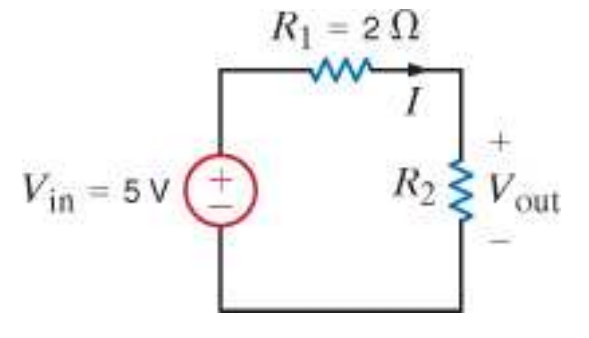
\includegraphics[width=4cm]{img/puisCircuit.png}
\includegraphics[width=6.5cm]{img/maxPuissance.png}
\caption{Graphique montrant l'évolution de la puissance dans une résistance}
\end{figure}

\subsubsection{Le quadripole à 2 accès}
\begin{wrapfigure}{r}{.45\textwidth}
\centering
\includegraphics[width=6.5cm]{img/quadri2.png}
\caption{Schéma classique d'un quadripole à 2 accès}
\end{wrapfigure}
Le quadripole à 2 accès se reposent sur 2 principes, il faut qu'il n'y ait aucune source indépendante interne $\rightarrow$ donc passif. Il faut également n'avoir que 2 accès, c'est à dire que la somme des entrées est nulle. Pour simplifier, il faut qu'on ait une entrée et sortie comprenant le même courant (voir schéma ci-contre).\\
Le but de cette représentation est une simplification de circuit. De plus, même si ce circuit n'est pas linéaire, on fait des petites variations autour d'une valeur rendant approximativement le circuit linéaire.\\

Ce type de quadripole peut être réalisé de 4 manières différentes détaillées ci-dessus.
\begin{figure}[H]
\centering
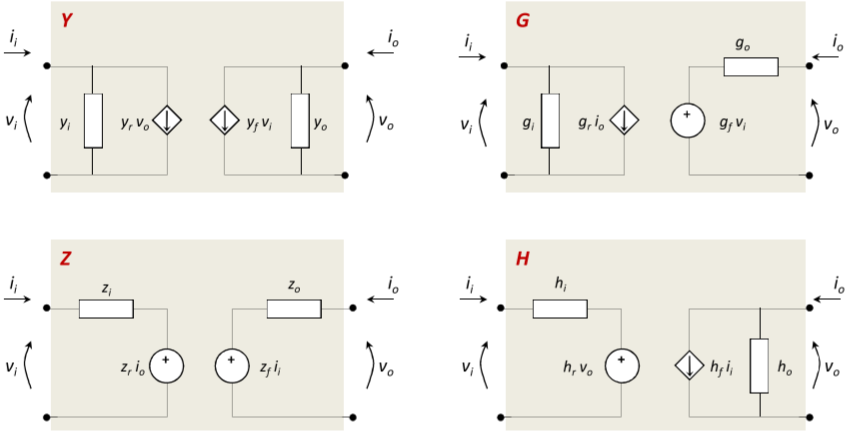
\includegraphics[width=10cm]{img/YZGH.png}
\caption{Les 4 types de quadripoles}
\end{figure}
On peut facilement représenter ces différents systèmes via des matrices détaillant le système voir \ref{Quadri}.
%insérer la matrice

\subsection{L'amplificateur opérationnelle}
L'amplificateur opérationnelle ou \textit{ampli op} est un composant qu'on retrouve abondamment en électronique.\\
On va éviter la saturation et contrôler l'ampli-op en réalisant une boucle de rétroaction négative à la borne $-$. Nous n'avons aucun courant qui rentre dans l'ampli-op dû à son impédance élevée. Il se peut qu'à la sortie de celle-ci, un faible courant puisse rentrer car l'impédance est plus faible.

\subsubsection{Buffer}
\begin{figure}[H]
\centering
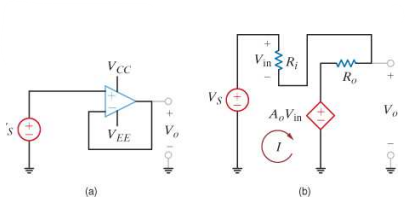
\includegraphics[width=6cm]{img/buffer.png}
\end{figure}
Permet de trier un maximum de courant sans changer la tension.
\begin{equation}
\frac{V_0}{V_S} = \frac{1}{1 + \frac{R_i}{R_o + A_o R_i}} \approx 1
\end{equation}
Et avec une ampli-op idéale, $A_0 \rightarrow \infty$, $R_i \rightarrow \infty$ et $R_o \rightarrow 0$.

\subsubsection{Inverseur}
\begin{figure}[H]
\centering
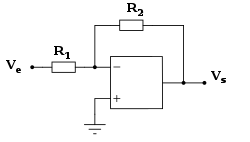
\includegraphics[width=5cm]{img/Aopinverting.svg.png}
\end{figure}
où $\frac{v_o}{v_s} \approx - \frac{R_2}{R_1}$.

\subsubsection{Non-inverseur}
\begin{figure}[H]
\centering
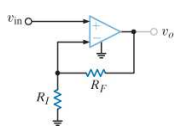
\includegraphics[width=5cm]{img/nonInv2.png}
\end{figure}
Où $\frac{v_o}{v_{in}} = 1 + \frac{R_F}{R_l}$.

\subsubsection{Différence}
\begin{figure}[H]
\centering
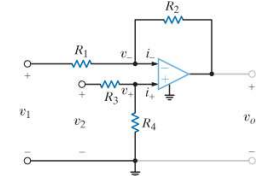
\includegraphics[width=6cm]{img/dif.png}
\end{figure}
Le but est de faire la différence entre deux tensions. 
\begin{equation}
v_o = \frac{R_1 + R_2}{R_1} \frac{R_4}{R_3 + R_4} v_2 - \frac{R_2}{R_1} v_1
\end{equation}

\subsubsection{Intégrateur}
\begin{figure}[H]
\centering
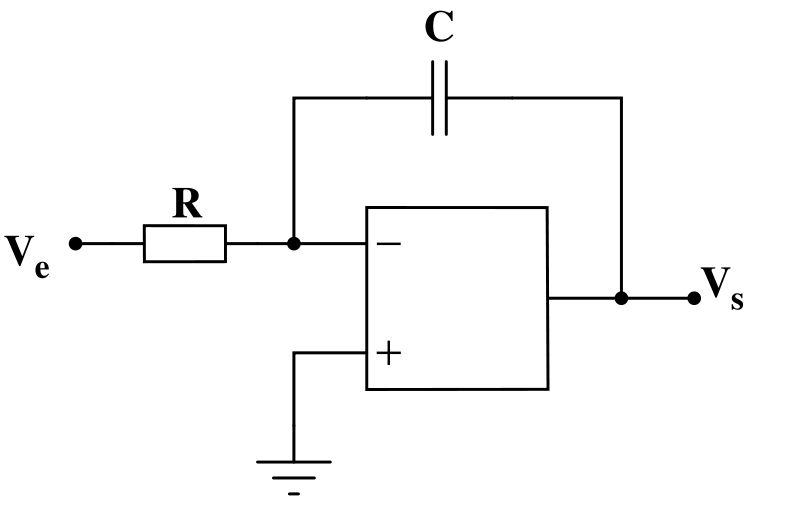
\includegraphics[width=5cm]{img/800px-Aopintegrating.svg.png}
\end{figure}
On doit parfois rajouter une résistance en parallèle de la capacité pour en faire un intégrateur à perte. On l'ajoute quand on n'a rien en aval du bloc.
\begin{equation}
V_{out} = - \frac{1}{RC} \int_{t = 0}^{t} V_{in} dt + V_{out} (0)
\end{equation}


\chapter{Signaux sinusoïdaux et phaseurs}
\section{Circuits en régime sinusoïdal}

\subsection{Circuit RC: rappel}
Dans cette partie, on s'intéressera surtout au circuit \textbf{RC}, il est donc bon de rappeler différentes formules:
\begin{align}
I_C(t) &= C \frac{dV_C(t)}{dt}\\
V_R(t) &= RI(t)\\
RC \frac{dV_C(t)}{dt} &= -(V_C(t)-V_S(t))\label{eq:RCsinus}
\end{align}

\begin{figure}[H]
\centering
\includegraphics[width=5cm]{img/RCsinus.png} \label{img:RCsinus}
\caption{Circuit RC en régime sinusoïdal}
\end{figure}

Il est à noter que l'équation \ref{eq:RCsinus} est une équation propre au circuit de la figure \ref{img:RCsinus}. Il est bon de remarquer que \textit{maintenant}, les courants et tension sont \textit{dépendantes du temps}. La \textit{constante de temps} est $\tau = RC$ et apparait dans la résolution de \textit{l'équation différentielle}.

\subsection{Circuit LC}
Voici les formules pou les circuits LC. (\textit{note}: on dirait que notre source de courant est une source de courant \textit{commandée} mais c'est bien une source de courant \textbf{non-commandée})
\begin{align}
V_L(t) &= L \frac{dI_L(t)}{dt}\\
V_L(t) &= GI_G(t)\\
GL \frac{dI_L(t)}{dt} &= -(I_L(t)-I_S(t))\label{eq:LCsinus}
\end{align}

\begin{figure}[H]
\centering
\includegraphics[width=4.6cm]{img/LCsinus.png} \label{img:LCsinus}
\caption{Circuit LC en régime sinusoïdal}
\end{figure}

Il est à noter que l'équation \ref{eq:LCsinus} est une équation propre au circuit de la figure \ref{img:LCsinus}. La \textit{constante de temps} est $\tau = \frac{L}{R}$

\subsection{Régime sinusoïdal}
Quelques notions à bien comprendre:
\begin{itemize}
\item La phase est établi par l'observateur car c'est lui qui définit "\textit{le début de la sinusoïdale}"
\item Un cosinus est un sinus \textit{déphasé} de $\frac{\pi}{2}$
\end{itemize}

\subsubsection{Analyse circuit RC}
Si on a une source de courant sinusoïdale:
\begin{align}
V_s(t) &= V_p cos(\omega t)\\
\omega_0 &= \frac{1}{\tau} = \frac{1}{RC}\\
\frac{1}{\omega_0}\frac{dV_c(t)}{dt} + V_c(t) &= V_p cos(\omega t) \label{eq:RCdiff}
\end{align}

L'équation \ref{eq:RCdiff} correspond à l'équation différentielle et à pour solution:

\begin{equation} 
\begin{cases}
V_C(0) = 0\\
V_C(t) = \frac{V_p}{\textcolor{blue}{\sqrt{1 + \frac{\omega^2}{\omega_0^2}}}} \Bigl[\textcolor{brown}{-cos(\varphi)e^{-\frac{t}{\tau}}} + \textcolor{green}{cos(\omega t + \varphi)} \Bigl] \label{eq:RCsol}
\end{cases} 
\end{equation}
L'équation \ref{eq:RCsol} nous indique plusieurs choses:
\begin{enumerate}
\item La partie en \textcolor{blue}{bleu} nous montre une atténuation du signal.
\item La partie en \textcolor{brown}{brun} nous montre une partie \textit{transitoire} dû à la capacité qui se charge doucement avant d'arriver à un état stable.
\item La partie en \textcolor{green}{vert} est le \textit{déphasage} du signal qui est créé par le caractère "\textit{dérivateur}" d'une capacité
\end{enumerate}

%finir de clarifier les 2 dernières slides de cette sous-section

\subsection{Les Phaseurs}
On utilise des \textbf{phaseurs} pour des circuits:
\begin{itemize}
\item \textit{linéaires}
\item  ne possédant \textit{qu'une source indépendante}
\item on a une source de fréquence $\omega/ 2\pi$
\item le circuit est \textit{en régime}
\end{itemize}

Donc tous les autres \textit{courants dépendants} ont
\begin{itemize}
\item une \textit{forme} ressemblant à la source
\item la \textit{même fréquence}
\item une \textit{amplitude différente} 
\item une \textit{phase différente}
\end{itemize}
Seulement si cela est respecté, alors on peut utiliser les \textbf{phaseurs}:
\begin{align}
\textbf{V} &= V_M e^{j\psi_V}\\
\textbf{I} &= I_M e^{j\psi_I}
\end{align}
En électricité, on représente le nombre complexe par $j$. $\psi$ représente les phases.\\
L'utilisation des \textit{phaseurs} vient de l'idée de la \textit{formule d'Euler} où quand on ajoute une partie imaginaire, cela n'affecte pas la partie \textit{réelle}. Donc on peut faire ceci:
\begin{equation}
\begin{cases}
A cos(\omega t + \varphi) \rightarrow A cos(\omega t + \varphi) + j A sin(\omega t + \varphi) \qquad -\frac{\pi}{2}  \geq \varphi \geq \frac{\pi}{2} \\
A cos(\omega t + \varphi) \rightarrow \bigr[ Ae^{j\varphi} \bigr]e^{j\omega t}
\end{cases} 
\end{equation}
Ici, la deuxième équation utilise des \textit{phaseurs} (mis entre parenthèses, l'utilisation de phaseurs va simplifier notre notation surtout en dérivée et intégrale:
\begin{align}
\frac{d}{dt}\bigr[ Ae^{j\varphi} \bigr]e^{j\omega t} &= \bigr[ j \omega Ae^{j\varphi} \bigr]e^{j\omega t} \\
\int \bigr[ Ae^{j\varphi} \bigr]e^{j\omega t} &= \bigr[ \frac{1}{j \omega} Ae^{j\varphi} \bigr]e^{j\omega t}
\end{align}

Il est important de se rappeler que lorsqu'on travaille en \textit{complexe}, multiplier par $j$ reviens à faire une rotation \textit{anti-horlogé} de $\frac{\pi}{2}$.

%clarifier la fin

\subsection{Analyse de circuits}
Passer en phaseur est un opération \textbf{linéaire} donc toutes les lois de \textit{Kirchoff} et théorèmes de la \textit{théorie des circuits} restent \textbf{valables}.

\begin{center}
\begin{tabular}{|c|c|c|c|}
\hline
Élément & Résistance & Inductance & Capacité\\
\hline 
Paramètre & $\textbf{Z} = R$ & $\textbf{Z} = j\omega L$ & $\textbf{Z} = \frac{1}{j \omega C}$\\
$\textbf{Z} = \frac{1}{\textbf{Y}}$ & $\textbf{Y} = \frac{1}{R}$ & $\textbf{Y} = \frac{1}{j \omega L}$ & $\textbf{Y} = j \omega C$ \\
\hline 
Équation constitutive & $V = \textbf{Z}I$ & $V = \textbf{Z}I$ & $V = \textbf{Z}I$\\
 & $I = \textbf{Y}V$ & $I = \textbf{Y}V$ & $I = \textbf{Y}V$\\
\hline
\end{tabular}
\end{center}

Pour des \textbf{dipôles}:
\begin{center}
\begin{tabular}{|c|c|}
\hline
\textbf{Impédance} d'un dipôle & \textbf{Admittance} d'un dipôle\\
\hline
$\textbf{V} = \textbf{ZI}$ & $\textbf{I} = \textbf{YV}$\\
\hline
$\textbf{Z} = \frac{\textbf{V}}{\textbf{I}} = \frac{|\textbf{V}|}{|\textbf{I}|}e^{j(arg(\textbf{V})-arg(\textbf{I})} = \frac{V}{I} e^{j{(\psi_V-\psi_I)}}$ & $\textbf{Y} = \frac{\textbf{I}}{\textbf{V}} = |\textbf{Y}|e^{j(arg(\textbf{Y}))} = Y e^{j{(\varphi)}}$\\
\hline
\end{tabular}
\end{center}

On a différente notation pour $\textbf{Z}$:
\begin{align}
\textbf{Z} &= |\textbf{Z}|e^{j arg(\textbf{Z})} = Z e^{j\varphi} \qquad \text{représentation polaire}\\
\textbf{Z} &= R +jX \qquad \text{représentation cartésienne}
\end{align}
\begin{wrapfigure}{r}{.5\textwidth}
\centering
\includegraphics[width=7cm]{img/impedance.png}
\end{wrapfigure}

R est la \textit{résistance} et X la \textit{réactance}. Si cette dernière est \textbf{négative}, on a affaire à une \textit{capacité}. Si elle est \textbf{positive}, il s'agit d'une \textit{inductance}

Donc on voit clairement que notre vecteur \textbf{Z} a une composante \textit{complexe} et \textit{réelle}. Et cela vaut de même pour le vecteur \textbf{Y}.

\subsubsection{Impédance de résistance pure}
\begin{itemize}
\item $\textbf{V} = R \textbf{I}$ et donc $\textbf{Z} = R$
\item Tension en phase: $\varphi = 0 \rightarrow $\textbf{V}$ = R I_{M} e^{j \psi_{I}}$
\item Admittance: $\textbf{Y} = G = \frac{1}{R}$ 
\end{itemize}

\subsubsection{Impédance d'inductance pure}
\begin{itemize}
\item $\textbf{V} = j \omega L \textbf{I}$ et donc $\textbf{Z} = j \omega L$
\item Tension en \textbf{avance} sur le courant: $\varphi = \frac{\pi}{2} \rightarrow \textbf{V} = \omega L I_M e^{j(\psi_I + \frac{\pi}{2})}$
\item Admittance: $\textbf{Y} = jB = \frac{1}{j \omega L}$ 
\end{itemize}


\subsubsection{Impédance de capacité pure}
\begin{itemize}
\item $\textbf{I} = j \omega C \textbf{V}$ et donc $\textbf{Y} = j \omega C$
\item Tension en retard sur le courant: $\varphi = \frac{-\pi}{2} \rightarrow \textbf{I} = \omega C V_M e^{\psi_V + \frac{\pi}{2}}$
\item Impédance: $\textbf{Z} = jX = \frac{1}{j \omega C}$ 
\end{itemize}
Attention à bien remarquer l'utilisation d'une impédance au lieu d'une admittance comme précédemment.

\subsubsection{Même dipôle}
\begin{figure}[H]
\centering
\includegraphics[width=7cm]{img/memeDipole.png}
\end{figure}

\subsection{Admittance équivalente à une impédance}
À une \textcolor{red}{fréquence précise}, tout dipôle en série peut être remplacé par un dipôle en parallèle.\\

En effet, il suffit de recréer le même vecteur. Dans le cas en \textbf{série}, on impose le courant donc:
\begin{align}
\textbf{$V_{R}$} &= |\textbf{Z}|cos(\varphi) \textbf{I} \rightarrow \textbf{Z} = R\\
\textbf{$V_{L}$} &= |\textbf{Z}|sin(\varphi) \textbf{I} \rightarrow \textbf{Z} = \omega L&
\end{align}
Et dans le second cas, on impose la tension au borne:
\begin{align}
\textbf{I} &= \textbf{V} \textbf{Y}\\
\textbf{$I_{R}$} &= \frac{1}{|\textbf{Z}|}cos(\varphi) \textbf{V} \rightarrow \textbf{Y} = \frac{1}{\textbf{Z}}\\
\textbf{$I_{L}$} &= \frac{|\textbf{Z}|}{sin(\varphi)} \textbf{V} \rightarrow \textbf{Y} = \frac{1}{\omega L} 
\end{align}
Il faut bien se rendre compte que cet équivalent est uniquement valable pour une \textcolor{red}{même fréquence}. Car le $|\textbf{Z}|$ varie ainsi que le déphasage $\varphi$. \\
Pour faire la différence quand on a des graphes comme ci-dessous, on peut voir que à basse fréquence (donc quasi DC) aucun courant ne passe dans la capacité pour un circuit en parallèle. Cela implique qu'on n'a pas de déphasage car tout le courant passe dans 	la résistance. De plus, l'impédance est quasi constante. (\textit{on peut prouver un équivalent la même chose pour le circuit en série})

\begin{figure}[H]
\centering
\includegraphics[width=7cm]{img/EquivalentRC.png}
\caption{En \textcolor{blue}{bleu} le circuit en série, en \textcolor{green}{vert} le circuit en parallèle}
\end{figure}

\subsection{Addition Impédance}
Comme dit au début du chapitre, on conserve toutes les lois classiques des circuits en courant continu. Cela implique que:
\begin{itemize}
\item Pour les impédances:
	\begin{itemize}
	\item On additionne simplement les impédances en série.
	\item On réalise la formule $\frac{1}{\frac{1}{Z_1} + ... + \frac{1}{Z_n}}$ pour des impédances en parallèle.
	\end{itemize}
\item Pour les admittances:
	\begin{itemize}
	\item On réalise la formule $\frac{1}{\frac{1}{Y_1} + ... + \frac{1}{Y_n}}$ pour des admittances en série.
	\item On additionne simplement les admittances en parallèle.
	\end{itemize}
\end{itemize}
Cette \textit{dualité} impédance-admittance est très utile et simplifie de nombreux calculs pour les circuits \textit{AC}.

\subsection{Thévenin et Norton}
On fait les mêmes démarches qu'en \textit{DC}, il faut faire attention aux impédances complexes et les sources de courants et tension qui sont des \textit{phaseurs}.

\subsection{Conseil}
La valeur efficace $= V_{RMS}$ et notre valeur de crête en sinusoïdale $= \sqrt{2}V_{RMS}$.\\
On calcule notre puissance en valeurs efficaces. La puissance active est la partie réelle et la puissance réactive est la partie complexe. La puissance complexe se calcule depuis les valeurs \textit{efficaces}.



\chapter{Comportement des circuits en domaine fréquentielle}
Nous avons déjà vu que la \textit{fréquence} influence notre \textit{impédance} et \textit{phase}.

\section{Diagramme de Bode}
Le Diagramme de Bode est une façon conventionnelle de représenter un circuit selon une évolution de la fréquence. Ce type de graphe utilise des axes logarithmiques avec en axe \textbf{X} la fréquence et en axe \textbf{Y} notre valeur d'intérêt (ici, un courant)

\begin{figure}[H]
\centering
\includegraphics[width=6.5cm]{img/BodeEx.png}
\caption{Exemple pour $\textbf{A} = A_0 \frac{1}{1 + \frac{j \omega}{\omega_0}}$} \label{BodeEx}
\end{figure}

\subsection{Info}
Il est important de ne pas oublie qu'un diagramme de \textit{Bode} est un diagramme qui est \textbf{logarithmique} et il faut en produire \textbf{2}, un pour l'\textbf{amplitude} et un pour la \textbf{phase}.\\

L'axe \textbf{X} est d'une entrée $log(\omega)$. Donc si on descend en-dessous de \textit{1Hz}, on tombe à $-\infty$ sur l'axe abscisses.

\subsection{Calculer}
\subsubsection{Amplitude} \label{AmplCalc}
L'exemple montré en \ref{BodeEx} est un exemple classique qu'on rencontre en circuit AC. La formule pour transformer \textbf{A} en $log$ est:
\begin{equation}
20log(\textbf{A}) = 20 log\Bigl(A_0\frac{1}{1+\frac{j\omega}{\omega_0}}\Bigl) = 20log(A_0) - 20log\Bigl(1+ \frac{j\omega}{\omega_0}\Bigl)
\end{equation}
Pour tracer un graphe il faut:
\begin{itemize}
\item Regarder quand $\omega < < \omega_0 \rightarrow$ ici on a donc une équation qui devient $\textbf{A} = A_0$
\item Regarde quand  $\omega > > \omega_0 \rightarrow$ On peut donc ignorer le $1$ au dénominateur. Ce qui devient donc $20log(A_0) - 20log(j\omega) + 20 log(\omega_0)$ Donc on a une droite qui "descend" de 20 dB par décade.
\end{itemize}

\subsubsection{Phase}
Le rapport d'argument de l'exemple \ref{BodeEx} est:
\begin{equation}
arg(H) =  arg(A_0) - arg\Bigl(1 + \frac{j\omega}{\omega_0}\Bigl)
\end{equation}
Donc on utilise le même principe qu'au point \ref{AmplCalc}:
\begin{itemize}
\item Regarder quand $\omega < < \omega_0 \rightarrow$ l'équation devient donc $arg(A_0)-arg(1) = 0$ donc on a aucun déphasage.
\item Regarder quand $\omega > > \omega_0 \rightarrow$ l'équation devient donc $arg(A_0) -arg\Bigl(\frac{j\omega}{\omega_0}\Bigl) = -\frac{\pi}{2}$
\end{itemize}

\subsubsection{Tracer}
Pour tracer notre graphe, on doit "\textit{arrondir}" les angles pour retranscrire plus le coté physique et réaliste.

\subsection{Interprétation}
Toujours en se basant sur \ref{BodeEx}, on est sur un "\textit{filtre passe-bas}". C'est même plus que ça car la valeur $A_0$ agit comme un amplificateur des basses fréquences. Et puis, on perd de plus en plus les hautes fréquences par un système \textit{intégrateur}.

\subsection{Modèle plus compliqué}
Pour cela, on répète autant de fois qu'il y a de $\omega_n$ l'opération. On retient que quand la fonction est au \textit{numérateur}, on croit. Au \textit{dénominateur}, on décroit.\\
Ainsi, on aurait un ensemble de courbe et de droite qu'on doit simplement sommer entre elle. (ne pas oublier d'arrondir les angles pour donner un côté plus réaliste)\\
La partie complexe est toujours renvoyer vers l'argument où là celle-ci aura un impact plutôt que sur l'amplitude !

\subsection{Formule générale}
L'équation du rapport de puissance est en général de forme:
\begin{equation}
A_V = \textcolor{red}{A_{V0}(j\omega)^{\pm N}}\frac{\textcolor{blue}{\Bigl(1 + \frac{j\omega}{\omega_1}\Bigl)} \textcolor{orange}{\Bigl( 1 + 2 j \xi_a \frac{\omega}{\omega_a} - \Bigl[ \frac{\omega}{\omega_a}\Bigl]^2 \Bigl)}}{\textcolor{blue}{\Bigl(1 + \frac{j\omega}{\omega_2}\Bigl)} \textcolor{orange}{\Bigl( 1 + 2 j \xi_b \frac{\omega}{\omega_b} - \Bigl[ \frac{\omega}{\omega_b}\Bigl]^2 \Bigl)}}
\end{equation}
\newpage
\begin{enumerate}
\item $\textcolor{red}{A_{V0}(j\omega)^{\pm N}}$:
	\begin{itemize}
	\item Amplitude: est une constante
	\item Phase: nous déphase de $\pm \frac{\pi}{2}$ en fonction de $\pm N$ et ce de manière rectiligne de 20 dB par décade.
	\end{itemize}
\item $\textcolor{blue}{\frac{\textcolor{blue}{\Bigl(1 + \frac{j\omega}{\omega_1}\Bigl)}}{\textcolor{blue}{\Bigl(1 + \frac{j\omega}{\omega_2}\Bigl)}}}$:
	\begin{itemize}
	\item Amplitude: au \textbf{dénominateur}, on est face à un filtre \textit{passe-bas}. Au \textbf{numérateur} on est face à un "amplificateur" \textbf{passe-haut}.
	\item Phase: au \textbf{dénominateur}, déphasage de $-\frac{\pi}{2}$ et déphasage de $\frac{\pi}{2}$ au \textbf{numérateur}.
	\end{itemize}
\item $\textcolor{orange}{\frac{\textcolor{orange}{\Bigl( 1 + 2 j \xi_a \frac{\omega}{\omega_a} - \Bigl[ \frac{\omega}{\omega_a}\Bigl]^2 \Bigl)}}{\textcolor{orange}{\Bigl( 1 + 2 j \xi_b \frac{\omega}{\omega_b} - \Bigl[ \frac{\omega}{\omega_b}\Bigl]^2 \Bigl)}}}$ cette partie est plus subtile et on doit s'intéresser au $\xi$, pour trouver les fréquences de coupure, on fait simplement un $\Delta$:
	\begin{enumerate}
		\item $\xi >  1$ (on suppose que $\omega_a < \omega_b$)
		\begin{itemize}
			\item Amplitude: une augmentation/diminution en 20dB par décade de $\omega_a \leq \omega \leq \omega_b$ puis de 40 dB à partir de $\omega_b$ si cela est au numérateur/dénominateur.
			\item Phase: Rotation de $\pi$ si au \textit{numérateur} ou rotation de $\pi$ au \textit{dénominateur}.
		\end{itemize}
		
		\item $\xi = 1$ (on suppose que $\omega_a < \omega_b$)
		\begin{itemize}
			\item Amplitude: une augmentation/diminution de 40 dB par décade à partir de $\omega_b = \omega_a$ si cela est au numérateur/dénominateur.
			\item Phase: Rotation de $\pi$ si au \textit{numérateur} ou rotation de $\pi$ au \textit{dénominateur}.
		\end{itemize}
		\item $0 \leq \xi < 1$ cas très spécial ! (on suppose que $\omega_a < \omega_b$) on un phénomène de résonance d'amplitude. \textit{overshoot}
		\begin{itemize}
			 \item Amplitude: comme au point (b) mais au centre, on une asymptote qui tend vers le bas/haut si c'est au numérateur/dénominateur.
			 \item Phase: changement de phase mais avec une pente plus raide autour du centre. voir \ref{XI}.
		\end{itemize}
	\end{enumerate}
\end{enumerate}
%enlever la double coloration 

\begin{figure}[H] 
\centering
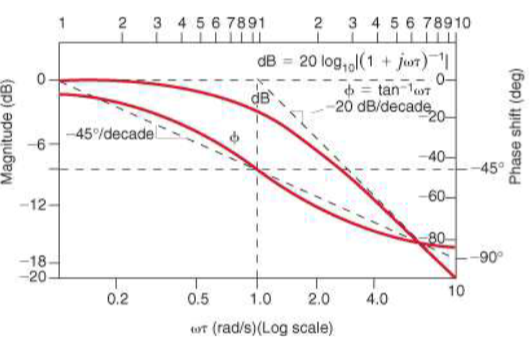
\includegraphics[width=7cm]{img/AmpXI.png}
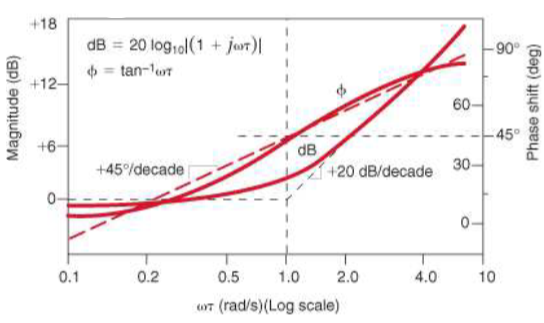
\includegraphics[width=7cm]{img/PhaseXI.png}
\caption{Amplitude et Phase pour le (c)}\label{XI}
\end{figure}

\section{Circuits résonants et filtrage}
\noindent
Maintenant, voyons des cas concrets de circuit RLC implémentant des courants AC.

\subsection{Circuits résonants}

\subsubsection{Circuits résonants en série}
Avec un circuit en série d'inductance, capacité et résistance, on a une impédance comme:
\begin{align*}
\textbf{Z} = R + j\omega L + \frac{1}{j \omega C} &= R + j \Bigr(\omega L - \frac{1}{\omega C} \Bigr)\\
\omega_0 &= \frac{1}{\sqrt{LC}}
\end{align*}
Pour être en résonance, il faut annuler la partie complexe. On nomme cette \textcolor{blue}{fréquence de résonance} $\omega_0$.\\
On établit aussi un \textcolor{blue}{facteur de qualité} d'un circuit qui indique si on possède une bonne bobine pour le circuit. De plus, on peut avoir un rapport du voltage de la résistance sur le voltage totale $V_R / V_1$:
\begin{align*}
Q &= \frac{\omega_0 L}{R}\\
\frac{V_R}{V_1} &= \frac{1}{1 + j Q(\omega/ \omega_0 - \omega_0 / \omega)}
\end{align*}

Ceci nous permet d'avoir des pics à des fréquences spécifiques. Avec cela, on va pouvoir créer des filtres (radio tuning, ...).

\begin{figure}[H]
\centering
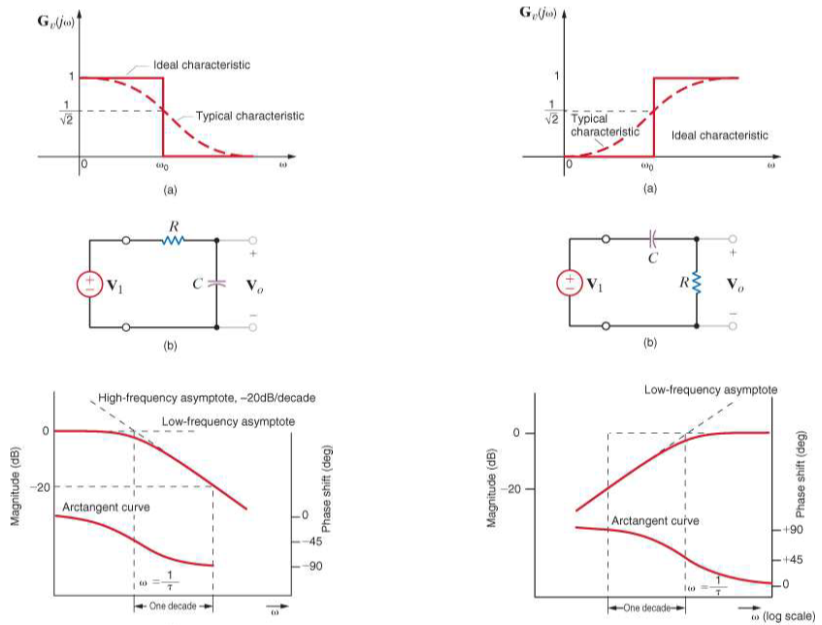
\includegraphics[width=8cm]{img/premierOrdre.png}
\caption{\textit{à gauche}: filtre du premier ordre passe-bas \textit{à droite}: filtre du premier ordre passe-haut}
\end{figure}

\begin{figure}[H]
\centering
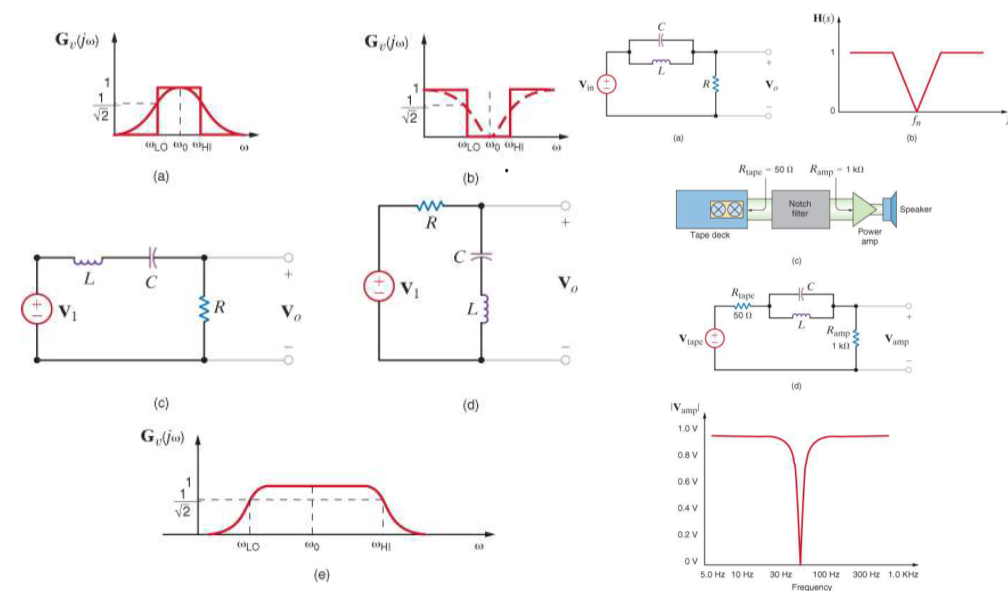
\includegraphics[width=9cm]{img/premierOrdre2.png}
\caption{\textit{à gauche}: passe-bande \textit{au milieu}: stop-bande \textit{à droite}: notch}
\end{figure}


\section{Conception des filtres} 
Les critères pour un filtre sont:
\begin{enumerate}
\item La fluctuation de bande passante: donc l'erreur d'amplification
\item La zone de transition: à quelle vitesse on passe de la zone passante à non-passante
\item La fluctuation de bande bloquante: on établit une marge d'erreur pour la partie bloquante
\end{enumerate}
On peut aussi remarquer un \textcolor{blue}{délai de groupe}. C'est la dérivé de la phase par rapport à $\omega$.\\
On va souvent créer des filtres en se basant sur des \textit{polynômes typiques}. On doit également choisir quelles caractéristiques on veut privilégier.

\subsection{Butterworth} \label{But}
Ce type de filtre à pour but d'avoir une fluctuation de la bande passant \textbf{quasiment nulle}.
\begin{align*}
G^2(\omega) = |H(j \omega )|^2 = \frac{G_0^2}{1+(\frac{\omega}{\omega_c})^{2n}} \Rightarrow H(j\omega ) = \frac{G_0}{B_n (\frac{j \omega }{\omega_c })}
\end{align*}

\begin{wrapfigure}{r}{.5\textwidth}
\centering
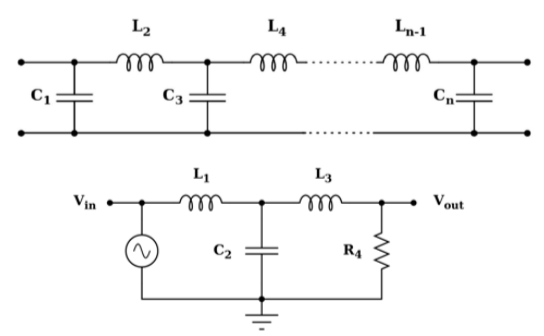
\includegraphics[width=6cm]{img/Butter.png}
\end{wrapfigure}
Son désavantage est son temps de transition plus ou moins long. De plus sa zone bloquante est plutôt stable mais n'annule pas efficacement les fréquences proche de la fréquence de coupure.\\
On l'implémente comme montré ci-contre.
\begin{align*}
C_k &= 2 sin \Bigl( \frac{(2k -1)}{2n} \pi \Bigl)\\
L_k &= 2 sin \Bigl( \frac{(2k -1)}{2n} \pi \Bigl)
\end{align*}
\begin{wrapfigure}{r}{.5\textwidth}
\centering
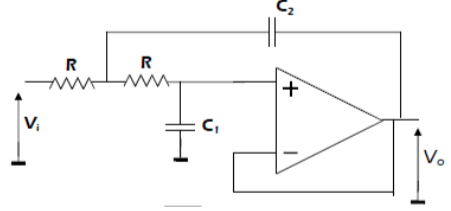
\includegraphics[width=6cm]{img/SallenKey.png}
\end{wrapfigure}
Il existe également des filtres de \textcolor{blue}{Sallen-Key} qui sont du \textit{deuxième ordre} ce qui permet des filtres plus fiables car ne dépendant pas de ce qu'il y a en aval.\\
En effet grâce à l'impédance d'entrée \textit{infini} des ampli-ops idéales, on ne sera jamais perturbé par les impédances en aval.

\subsection{Chebyshev}
\begin{wrapfigure}{r}{.5\textwidth}
\centering
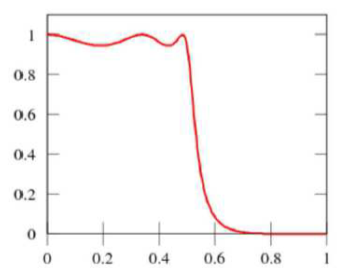
\includegraphics[width=6cm]{img/Cheby.png}
\end{wrapfigure}
L'avantage de ces filtres est qu'on a une zone de transition plus raide que Butterworth (\ref{But}) mais on a de plus fortes oscillations en bande passante.


\subsection{Bessel}
L'avantage des filtres de \textit{Bessel} est qu'il minimise la distorsion de la zone passante tout en ayant un délai de groupe \textbf{constant}.
\begin{align*}
H(s) &= \frac{\theta_n (0) }{\theta_n (\frac{s}{\omega_0 })}\\
n &= 1; s+1\\
n &= 2; s^2 + 3s + 3\\
n &= 3; s^3 + 6 s^2 + 15s + 15
\end{align*}
\begin{figure}[H]
\centering
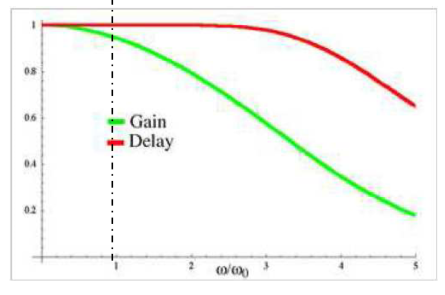
\includegraphics[width=7cm]{img/Bessel.png}
\caption{Filtre de Bessel}
\end{figure}

\section{Rétroaction et circuits en boucle fermée}

\subsection{Rétroaction}
\begin{wrapfigure}{r}{.5\textwidth}
\centering
\includegraphics[width=7cm]{img/Bloc.png} \label{img:ampli}
\end{wrapfigure}
Au lieu de régler quelque chose basé sur des instructions pré-déterminés, on va prendre des mesures et les effets d'un système pour pouvoir ajuster celui-ci.\\
Ceci rend notre machine plus efficace et permet à celle-ci de s'adapter peu importe le milieu.\\
Ci-contre un exemple en \textit{schéma-bloc} d'un système en \textcolor{blue}{boucle fermée}\\
\begin{itemize}
\item Chaine directe: correspond à un gain en puissance important
\item Chaine retour: l'ensemble des capteurs qui permettent de fournir une image du résultat du système
\item Soustracteur: permet de faire la différence entre ce qu'on fournit et le résultat ce qui permet d'être plus précis et à s'adapter
\end{itemize}

\subsubsection{Amplificateur opérationnelle}
Dans le monde réelle, on implémente ce type de système avec des \textbf{ampli-ops}. Elles ont un gain qui varie aux alentours de $10^5$.\\
Mais en boucle avec rétroaction \textit{négative} on peut fixer ce gain.
\begin{figure}[H]
\centering
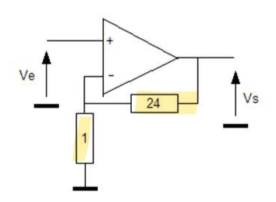
\includegraphics[width=7cm]{img/ampli.png} 
\end{figure}
Et donc le gain est $\frac{1}{24+1}$


\subsection{Représentation Schéma-Bloc}

\subsubsection{Fonction de transfert}
On a en entrée $E(j\omega)$ et le bloc de transfert $T(j\omega)$ nous donne $S(j\omega) = T(j\omega) . E(j\omega)$.\\
On peut remplacer les $j \omega$ par $s$ (voir chapitre \ref{Laplace})\\
On retrouve ce genre de bloc dans les \textit{amplificateurs, filtres, intégrateurs, ...}

\subsubsection{Soustracteur} 
On le représente par une boule (\ref{img:ampli}) et permet de faire la différence entre deux signaux.

\subsubsection{Mesure}
C'est une utilisation de plusieurs fonctions de transfert pour mesurer différentes choses.

\subsubsection{Déplacer}
Il n'y a pas qu'une seule configuration qui produit un résultat. On peut intervertir des blocs et les modifier pour avoir en sortie et en entrée les mêmes choses.

\subsubsection{Forme canonique}
\begin{figure}[H]
\centering
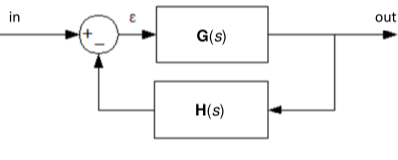
\includegraphics[width=6cm]{img/Bloc2.png}
\end{figure}
On peut voir ce système comme:
\begin{align*}
T_{bf}(s) = \frac{1}{H(s)}.\frac{G(s) . H(s)}{1 + G(s). H(s)} = T_{ideal} (s) . \frac{T_{bo}(s)}{1+T_{bo}(s)} = T_{ideal} (s) . \frac{1}{1 + \frac{1}{T_{bo}(s)}}
\end{align*}
Dans un monde idéal, le gain $G(s)$ tend vers $\infty$. Ainsi la fonction de transfert \textit{idéal} vaut donc $T_{ideal}(s) = 1/H(s)$


\subsection{Bode}
\subsubsection{Montage non-inverseur}
\begin{wrapfigure}{r}{.5\textwidth}
\centering
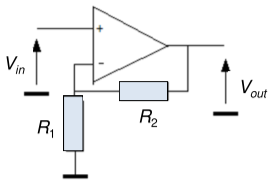
\includegraphics[width=6cm]{img/nonInv.png}
\caption{Montage non-inverseur}
\end{wrapfigure}
Ce type de montage a pour fonction de transfert selon $\omega$:
\begin{align*}
G(j \omega) = G_0 \frac{1}{1 + \frac{j\omega}{\omega_0}}
\end{align*}
Et la rétroaction est:
\begin{align*}
H(s) &= \beta^{-1}\\
\frac{V_{out}}{V_{in}} = \frac{G(j\omega)}{1 + \beta^{-1} G(j \omega)} &= \frac{1}{\beta^{-1}} \frac{\beta^{-1}G(j\omega)}{1 + \beta^{-1} G(j \omega)}\\
\Rightarrow T_{bf}(j \omega) &= \frac{1}{H} \frac{T_{bo}(j \omega)}{1 + T_{bo} (j \omega)}
\end{align*}
Donc on a une fonction constante jusqu'à $\omega_0$ et qui décroit de 20 dB par décade et tombe à 0 à $\omega = GBW$. GBW correspond au \textbf{Gain BandWidth} qui est une caractéristique propre à l'ampli-op.\\
Il est impossible de réaliser un montage non-inverseur de gain $\beta$ à une fréquence supérieure à $GBW/\beta$.
\begin{align*}
\omega_{0, bf} T_{0,bf} = \omega_{0, bf} \beta = \omega_0 G_0
\end{align*}

\subsubsection{Montage inverseur}
\begin{wrapfigure}{r}{.5\textwidth}
\centering
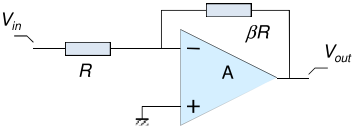
\includegraphics[width=5cm]{img/inv.png}
\caption{Montage inverseur}
\end{wrapfigure}
Ce type de montage a pour fonction de transfert selon $\omega$:
\begin{align*}
G(j \omega) = G_0 \frac{1}{1 + \frac{j\omega}{\omega_0}}
\end{align*}
Pour établir la rétroaction $H(s)$ cela est plus compliqué et moins direct
\begin{align*}
V_{in} - V_{-} &= \frac{V_{-}-V_{out}}{\beta} & 
V_{out} &= -G(j\omega) V_{-} & \frac{V_{out}}{V_{in}} &= - \frac{\frac{1}{1 + \frac{j \omega}{\omega_0}}}{1+ \beta + G_0 \frac{1}{1 + \frac{j \omega}{\omega_0}}}
\end{align*}
Ceci nous donne donc un rapport de tension:
\begin{align*}
\frac{V_{out}}{V_{in}} &= \frac{G_0 \beta}{1 + \beta + G_0} \frac{1}{1 + \frac{j\omega ( 1 + \beta)}{(1 + \beta + G_0) \omega_0}}\\
& \cong \frac{G_0 \beta}{1 + \beta + G_0} \frac{1}{1 + \frac{j \omega G_0 \beta}{(1 + \beta + G_0) G_0 \omega_0}} \equiv T_{0, bf} \frac{1}{1 + \frac{j \omega}{\omega_0 G_0 / T_{0, bf}}}\\
\omega_{0, bf} &=  \frac{\omega_0 G_0}{|T_{0, bf}|} = \frac{\omega_0 G_0}{\beta} \Rightarrow \beta \omega_{0, bf} = GBW
\end{align*}
Il est impossible de réaliser un montage non-inverseur de gain $\beta$ à une fréquence supérieure à $GBW/\beta$.

\subsubsection{Produit amortisseur-fréquence de coupure (second ordre)}
On a une expression du gain en boucle ouverte du second ordre typique:
\begin{align*}
G(j \omega) &= G_0 \frac{1}{1 + 2 j \xi \frac{\omega}{\omega_0} - \Bigr( \frac{\omega}{\omega_0} \Bigr)^2}
\end{align*}
Si on est en \textcolor{blue}{boucle fermée}, le produit invariant est $\xi \omega_0$:
\begin{align*}
\xi_{bf} &= \frac{\xi}{\sqrt{1 + G_0}} & \omega_{0, bf} &= \omega_0 \sqrt{1 + G_0}
\end{align*}
Il faut bien régler l'amortissement car on peut soit rendre le système \textit{sur amorti} et donc oscillatoire amorti ou bien \textit{sous amorti} et le système est trop réactif donc instable. 
\begin{figure}[H]
\centering
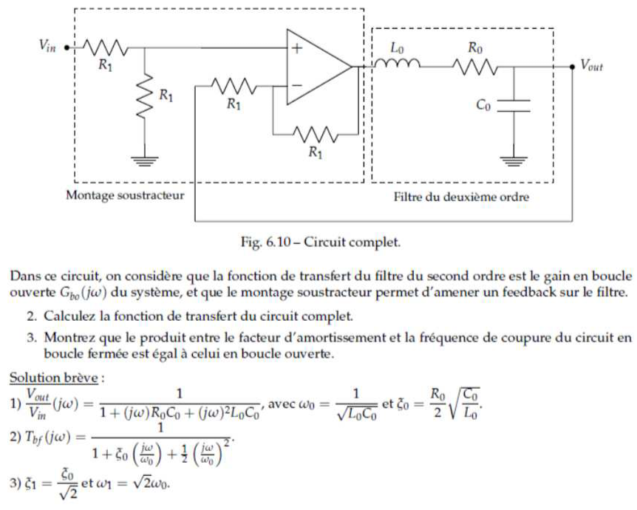
\includegraphics[width=10cm]{img/amortissement.png}
\caption{Système complet}
\end{figure}

\subsection{Conseils}
On ne peut plus considérer que $V_{i+} = V_{i-}$, on a que $\frac{V_o}{V_{i+} - V_{i-}}$ ce qui revient à:
\begin{equation}
V_o = G(j \omega ) ( V_{in} - V_{-})
\end{equation}


\section{Quadripôles} \label{Quadri}
\subsection{Rappels}
\begin{wrapfigure}{r}{.5\textwidth}
\centering
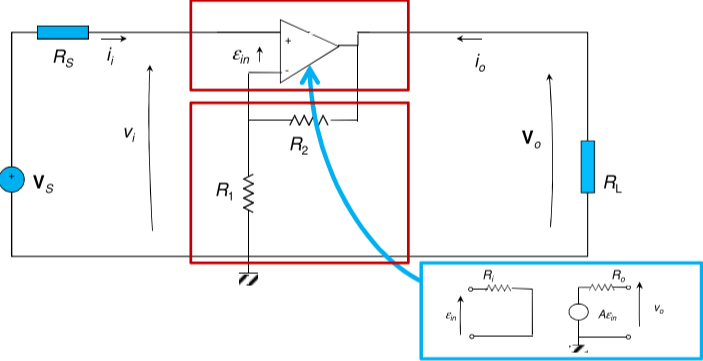
\includegraphics[width=8cm]{img/QuadriAmp.png}
\end{wrapfigure}
On peut simplifier des montages avec des ampli-ops en quadripôles. On remplace donc le montage en rouge ci-contre par le quadripôle en bleu.\\
Donc on les utilise lorsqu'on fait des opérations sur des signaux avec une idée de \textit{input} et \textit{output}.\\
Un \textcolor{blue}{accès} implique 2 bornes. Pour un \textit{dipôle} c'est simplement Thévenin et Norton (\ref{Th}). Pour un \textbf{quadripôle} à deux accès, on réalise des représentations \textit{équivalentes} $\textbf{Y, Z, G, H}$ (on ne peut pas avoir de sources indépendantes).

\subsubsection{Quadripôle}
Les conditions:
\begin{itemize}
\item Pas de source indépendante interne
\item Deux accès
\item On impose une des deux bornes avec une source de tension
\end{itemize}

\subsubsection{Équivalence}
Entre les 4 représentations, on a une équivalence et on ignore la structure et les variables internes. Il existe également des relations transitives comme ci-dessous.
\begin{figure}[H]
\centering
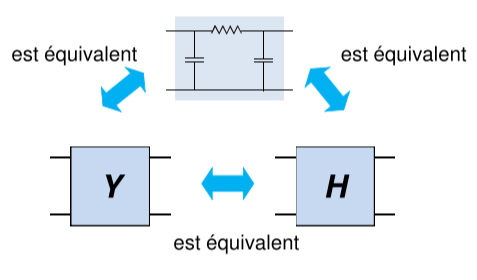
\includegraphics[width=7cm]{img/Trans.png} \label{img:trans}
\caption{Solution transitive au milieu}
\end{figure}

\subsection{L'équivalence}
On va toujours essayer de transformer un circuit complexe en un circuit quadripôles comme ci-dessous.
\begin{figure}[H]
\centering
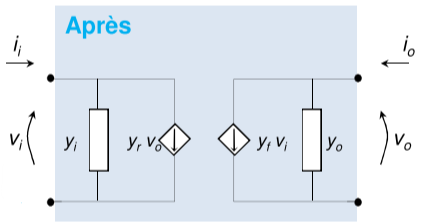
\includegraphics[width=6cm]{img/Transfo.png}
\end{figure}

\begin{center}
\begin{tabular}{|m {3cm}| m {4cm}| m {6cm}|}
\hline
Représentation & Formule & Définition\\
\hline
\textbf{Y} Admittances (transadmittances) & $\begin{bmatrix}
i_i\\ i_o
\end{bmatrix} = \begin{bmatrix}
y_i & y_r\\ y_f & y_o
\end{bmatrix}  \begin{bmatrix}
v_i\\ v_o
\end{bmatrix}$ & $y_i$: admittance d'entrée \newline $y_r$: transadmittance inverse (\textit{reverse}) \newline $y_f$: transadmittance directe (\textit{forward}) \newline $y_o$: admittance de sortie\\
\hline
\textbf{Z} impédances (transimpédances) & $\begin{bmatrix}
v_i\\ v_o
\end{bmatrix} = \begin{bmatrix}
z_i & z_r\\ z_f & z_o
\end{bmatrix}  \begin{bmatrix}
i_i\\ i_o
\end{bmatrix}$ & $z_i$: impédance d'entrée \newline $z_r$: transimpédance inverse (\textit{reverse}) \newline $z_f$: transimpédance directe (\textit{forward}) \newline $z_o$: impédance de sortie\\
\hline
\textbf{G} hybride & $\begin{bmatrix}
i_i\\ v_o
\end{bmatrix} = \begin{bmatrix}
g_i & g_r\\ g_f & g_o
\end{bmatrix}  \begin{bmatrix}
v_i\\ i_o
\end{bmatrix}$ & $g_i$: admittance d'entrée \newline $g_r$: gain en courant \newline $g_f$: gain en tension \newline $g_o$: impédance de sortie\\
\hline
\textbf{H} hybride & $\begin{bmatrix}
v_i\\ i_o
\end{bmatrix} = \begin{bmatrix}
h_i & h_r\\ h_f & h_o
\end{bmatrix}  \begin{bmatrix}
i_i \\ v_o
\end{bmatrix}$ & $h_i$: impédance d'entrée \newline $h_r$: gain en tension \newline $h_f$: gain en courant \newline $h_o$: admittance de sortie\\
\hline
\end{tabular}
\end{center}
\subsubsection{Représentation via Kirchhoff}
On peut voir les quadripoles comme des sources \textit{imparfaites}:
\begin{itemize}
\item Courant + admittance parasite (type Norton)
\item Tension + impédance parasite (type Thévenin)
\item Source commandée: influence d'un accès sur l'autre
\item Algèbre ou réseau de Kirchoff
\end{itemize} 
\begin{figure}[H]
\centering
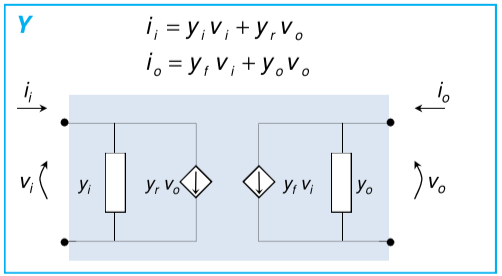
\includegraphics[width=7cm]{img/Ytransfo.png}
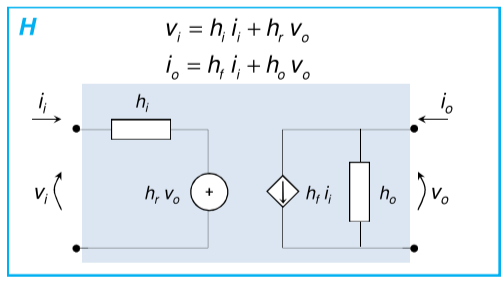
\includegraphics[width=7cm]{img/Htransfo.png}
\end{figure}
Pour passer de \textbf{Y} à \textbf{Z} on passe de Norton à Thévenin et de \textbf{H} à \textbf{G} on passe de Norton à Thévenin pour la \textit{droite} et de Thévenin à Norton pour la \textit{gauche}.

\subsection{Déterminer les coefficients}
Par exemple, pour un système \textbf{Y}, on peut montrer par algèbre que:
\begin{align*}
y_i &= \frac{i_i}{v_i} \biggl\vert_{v_o=0}\\
i_i &= y_i i + y_r v_o
\end{align*}
En effet, en mettant les bornes de sortie en court circuit, on peut ainsi déterminer $y_i$. Ainsi, on fait passer un courant $v_i$ qui est bien déterminé. On réalise des procédures similaires pour tous les coefficients.

\subsubsection{Règle}
\begin{enumerate}
\item Redessiner le schéma pour \textit{chaque coefficient}.
\item Appliquer les conditions de définition.
\item Source de \textit{test} pour la variable indépendante.
\item Déterminer la variable dépendante.
\item Calculer le coefficient.
\end{enumerate}

\subsection{Changement de représentation}
Cette partie renvoie directement à l'image \ref{img:trans}. Pour passer de \textbf{Y} à \textbf{H} on peut soit utiliser l'algèbre linéaire ou trouver des coefficients de \textbf{H} en partant de \textbf{Y}.

\subsubsection{Algèbre linéaire}
On connait:
\begin{align*}
i_i &= y_i v_i + y_r v_o\\
i_o &= y_f v_i + y_o v_o
\end{align*}
On veut trouver $v_i$ et $i_o$ en fonction de $i_i$ et $v_o$:
\begin{align*}
v_i &= h_i i_i + h_r v_o &
i_o &= h_f i_i + y_o v_o &
[H] &= \frac{1}{y_i} \begin{bmatrix}
1 & -y_r\\
y_f & \Delta^y
\end{bmatrix}
\end{align*}

\subsubsection{Coefficients}
On peut appliquer la règle de détermination des coefficients sur le schéma équivalent Y. On se rend compte qu'il faut utiliser la technique matricielle de temps en temps car peut vite être très lourde.
\begin{figure}[H]
\centering
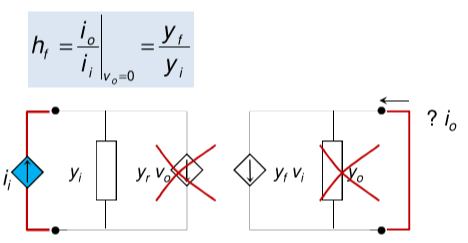
\includegraphics[width=7cm]{img/HYcoeff.png}
\end{figure}

\subsubsection{Conversion}
\begin{figure}[H]
\centering
\includegraphics[width=11cm]{img/Conversion.png}
\end{figure}
\begin{align*}
Z &= Y^{-1} & Y&= Z^{-1} & G &= H^{-1} & H &= G^{-1}
\end{align*}

\subsection{Association de quadripôle}
\begin{figure}[H]
\centering
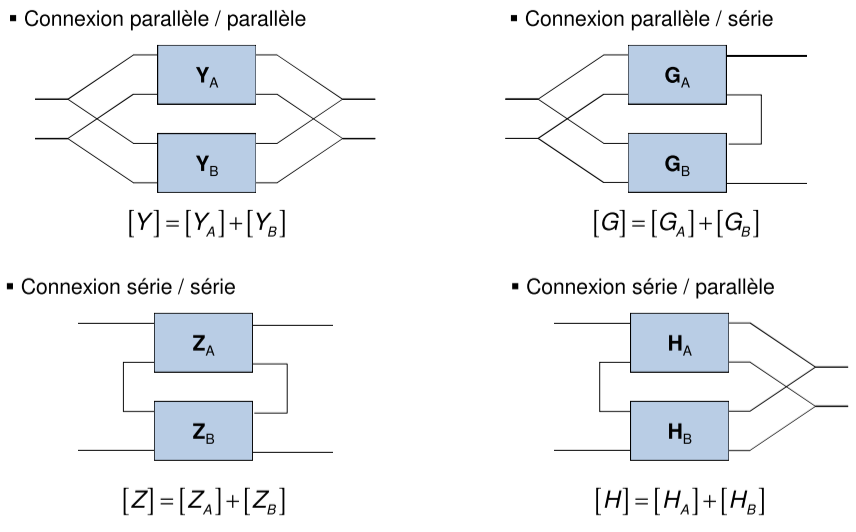
\includegraphics[width=10cm]{img/Assoc.png}
\end{figure}


\subsection{Quadripôle chargé}
\begin{figure}[H]
\centering
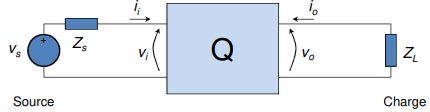
\includegraphics[width=7cm]{img/quadriCharge.png}
\end{figure}
C'est un quadripôle qui est entre une source $v_s$ avec $Z_s$ et une charge $Z_L$. De plus, on connait une des ses représentations.\\
On doit avoir une relation entre les variables externes en présence de $Z_s$ et $Z_L$. Il en existe 4:
\begin{enumerate}
\item \underline{Impédance d'entrée $Z_{in}$:} coefficient de $i_i$ dans l'expression de $v_i$, $Z_{in} = \frac{v_i}{i_i}$, dépend de $Z_L$.
\item \underline{Impédance de sortie $Z_{out}$:} coefficient de $i_o$ dans l'expression de $v_o$, $Z_{out} = \frac{v_o}{i_o}$, dépend de $Z_S$.
\item \underline{Gain en tension direct $A_{vf}$:} coefficient de $v_i$ dans l'expression de $v_o$, $A_{vf} = \frac{v_o}{v_i}$, dépend de $Z_L$.
\item \underline{Gain en courant direct $A_{if}$:} coefficient de $i_i$ dans l'expression de $v_o$, $A_{if} = \frac{i_o}{i_i}$, dépend de $Z_L$.
\end{enumerate}

On peut voir que $A_{vf}$, $A_{if}$ et $Z_{in}$ dépendent de $Z_L$, on a une répétition.\\
Pour déterminer les \textbf{caractéristiques externes} on va:
\begin{itemize}
\item On met une source de test pour la variable indépendante à l'un des accès
\item On charge l'autre accès par l'impédance correspondante ($Z_S$ ou $Z_L$)
\item On détermine la variable \textit{dépendante}
\item On calcule le coefficient
\end{itemize}
Pour trouver $Z_{out}$ on impose que $v_s = 0$.

\begin{figure}[H]
\centering
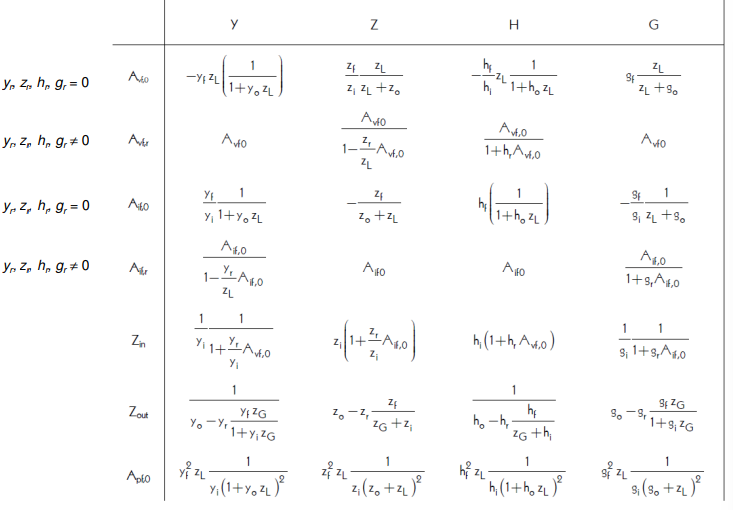
\includegraphics[width=14cm]{img/quadriTable.png}
\caption{Table des caractéristiques externes}
\end{figure}


\chapter{Puissance}
\section{Instantanée, moyenne et effective}

\subsection{Instantanée}
Une puissance est générée par le déplacement d'une charge $dq$ d'un point A vers B. On voit cela comme une énergie \textit{potentielle}. Donc au point X cela vaut $dq V_X$. Le déplacement crée un \textcolor{blue}{Travail} (\textit{Work}): $dW = dq (V_A - V_B)$. On fait un \textit{échange} de puissance avec le monde extérieur:
\begin{align*}
p &= \frac{dW}{dt} = \frac{dq}{dt}(V_A - V_B) = iv\\
p(t) &= v(t) i(t) \quad \text{Peut dépendre du temps}
\end{align*}
Dans les normes de ce cours, un dipôle \textcolor{red}{absorbe} de la puissance si le courant et la tension sont positifs ou négatifs.\\
On stocke cette énergie sous 2 forme.
\begin{enumerate}
\item Stocké sous forme d'énergie électrostatique (ex: capacité)
\item Stocké sous forme d'énergie magnétique (ex: inductance/self)
\end{enumerate}
Et on dissipe la puissance sous forme de chaleur pour une résistance ou en énergie mécanique pour un moteur électrique.\\

On dit qu'on \textbf{fournit} de la puissance si la tension est négative et le courant positif ou inversement. Donc on doit \textbf{générer} une puissance depuis une autre source (\textit{générateur de tension, capacité se vidant, ...})

\subsection{Moyenne}
Dans une résistance, la puissance est \textbf{toujours positive}. En effet, une résistance ne peut fournir de la puissance donc sa puissance moyenne est toujours positive.\\
Son voltage vaut: $v(t) = R i(t)$ et sa puissance \textcolor{blue}{instantanée} vaut donc $p(t) = R i^2(t)$ donc $p(t) = \frac{v^2(t)}{R}$.\\
La puissance moyenne se calcule via:
\begin{align*}
P_{moy} \triangleq \frac{1}{T} \int_{t_0}^{t_0 + T} p(t) dt = \frac{1}{T}\int_{t_0}^{t_0 + T} R i^2 (t) dt
\end{align*}
le $T$ correspond à une \textit{période} de notre signal d'entrée (alimentation).

\subsection{Valeur efficace}

\subsubsection{Courant}
Pour le courant \textit{continu}, on le nomme $I_{eff}$. Ainsi, la \textbf{puissance dissipée} dans la résistance vaut donc $R I_{eff}^2 = P_{moy}$.
\begin{align*}
I_{eff} = \sqrt{\frac{P_{moy}}{R}} = \sqrt{\frac{1}{T}\int_{t_0}^{t_0 + T} i^2 (t) dt}
\end{align*}

\subsubsection{Tension}
La tension \textit{continu}, on la nomme $V_{eff}$. Ainsi, la \textbf{puissance dissipée} dans la résistance $V_{eff}^2 / R = P_{moy}$.
\begin{align*}
V_{eff} = \sqrt{R P_{moy}} = \sqrt{\frac{1}{T}\int_{t_0}^{t_0 + T} v^2 (t) dt}
\end{align*}

\subsection{Courant sinusoïdal}
Si on a une pulsation de $\omega$ et une valeur de \textbf{crête} de $I_{max}$ et non déphasé, notre courant vaut: $i(t)= I_{max} cos(\omega t)$\\
Toujours avec une \textit{résistance}, sa puissance vaut donc:
\begin{align*}
p(t) &= R I_{max}^2 cos^2(\omega t)\\
&= \frac{R I_{max}^2}{2} (cos(2 \omega t) + 1)\\
&= P_{moy} (cos (2 \omega t ) +1 )\\
P_{moy} &= \frac{R I_{max}^2}{2} = R \left( \frac{I_{max}}{\sqrt{2}} \right)^2
\end{align*}
Pour ce type de courant et tension, on peut établir ces égalités:
\begin{align*}
I_{eff} &= \frac{I_{max}}{\sqrt{2}} & V_{eff} &= \frac{V_{max}}{\sqrt{2}}
\end{align*}

\subsubsection{Impédance quelconque}
On a une valeur de crête $I_{max}$ et $V_{max}$ qui ont la même pulsation de $\omega$ et une phase de $\varphi_i$ et $\varphi_v$ respectivement.\\
La puissance instantanée s'obtient ainsi:
\begin{align*}
p(t) &= V_{max}I_{max}cos(\omega t + \varphi_v) cos(\omega t + \varphi_i)
&= \frac{1}{2}V_{max}I_{max} [cos(\varphi_v -\varphi_i) + cos(2 \omega t + \varphi_v + \varphi_i)]
\end{align*}
On voit bien qu'on a donc un terme \textcolor{red}{constant} à gauche et un terme qui \textcolor{blue}{fluctue} à droite en fonction de la pulsation $2 \omega$\\
Ainsi, la puissance moyenne (par la propriété des cosinus) vaut le terme \textcolor{red}{constant}:
\begin{align*}
P_{moy} &= \frac{1}{2}V_{max}I_{max} cos(\varphi_v -\varphi_i) = V_{eff}I_{eff}cos(\varphi_v -\varphi_i)
\end{align*}

\section{Puissance active, réactive et apparente}
\subsection{Impédance quelconque}
On va tout d'abord transformer notre courant \textit{sinusoïdal} en phaseur: $\overline{I} = I_{max}e^{j\varphi_i}$\\
Comme nous sommes en impédance quelconque, cela signifie que: $\overline{Z} = R + j X = Z e^{j \varphi}$ petit rappel:
\begin{align*}
X &= \omega L & \varphi &= atan(\frac{X}{R}) & R &= Z cos(\varphi)\\
X &=  -\frac{1}{\omega C} & Z &= \sqrt{R^2 + X^2} & X &= Z sin(\varphi)
\end{align*}
Donc on peut en tirer ces équations en régime permanent:
\begin{align*}
\overline{V} &= \overline{Z} \overline{I}  = Z I_{max}e^{j (\varphi_i + \varphi)} & &\Rightarrow & \overline{V} &= V_{max}e^{j\varphi_v}\\
v(t) &= Ri(t) + L \frac{di(t)}{dt} & &\Rightarrow & v(t) &= Z I_{max} cos(\omega t + \varphi_i + \varphi)\\
& & i(t) &= C\frac{d}{dt}[v(t) -Ri(t)] & &
\end{align*}
La puissance instantanée vaut donc:
\begin{align*}
p(t) &= v(t) i(t) & p(t) &= V_{eff} I_{eff}(cos(\varphi_v - \varphi_i) + cos(2 \omega t + \varphi_v + \varphi_i ))\\
p(t) &= ZI_{eff}^2(cos(\varphi ) + cos(2 \omega t + \varphi + 2\varphi_i )) & p(t) &= RI_{eff}^2 + V_{eff}I_{eff} cos(2 \omega t + \varphi + 2\varphi_i )
\end{align*}

\subsubsection{Puissance active}
La puissance moyenne nous indique la puissance fournit au dipôle mais la puissance \textcolor{red}{active} indique un échange \textbf{unidirectionnel} de l'énergie entre la source et une charge (par exemple la résistance ici)
\begin{equation}
P \triangleq V_{eff} I_{eff} cos(\varphi) = R I_{eff}^2
\end{equation}

\subsubsection{Puissance apparente}
Son amplitude de la composante est fluctuante et s'écrit $S$ en \textbf{Volt ampère}:
\begin{align*}
S \triangleq V_{eff} I_{eff} = Z I_{eff}^2
\end{align*}

\subsubsection{Puissance réactive}
Traduit un échange \textbf{bidirectionnel} d'énergie entre une source et une charge (donc ici stocké et transmis depuis la \textit{réactance} \textcolor{blue}{$X$}. Cela s'écrit $Q$ en \textbf{Volt ampère réactif}. On ne peut utiliser cela que en régime \textcolor{red}{sinusoïdal}:
\begin{align*}
Q &\triangleq V_{eff} I_{eff} sin(\varphi) = XI_{eff}^2
S &= \sqrt{P^2 + Q^2}
\end{align*}

\subsection{Résistance pure - Courant imposé}
Ainsi, notre tension en régime permanent est parallèle au courant comme suit:
\begin{align*}
\overline{V} &= R \overline{I} & \overline{V} &= V_{max}e^{j \varphi_v} \qquad (V_{max} = R I_{max}, \quad \varphi_v = \varphi_i)\\
v(t) &= R i(t) & v(t) &= R I_{max} cos(\omega t + \varphi_i)
\end{align*} 

\begin{center}
\begin{tabular}{|m {3.5cm}| m {3.5cm}| m {3.5cm}| m {3.5cm}|}
\hline
Puissance active & Puissance apparente & Puissance réactive & Propriété\\
\hline
$P = RI_{eff}^2$ & $S = RI_{eff}^2$ & $Q = 0$ & $S = P$\\
\hline
\end{tabular}
\end{center}

\subsection{Inductance pure - Courant imposé}
Comme notre phase de la tension est en avance de $\frac{\pi}{2}$ par rapport à la tension, notre tension instantanée va valoir:
\begin{equation}
p(t) = \omega L I_{eff}^2 cos \left(2 \omega t + 2 \psi_i + \frac{\pi}{2} \right)
\end{equation}

\begin{center}
\begin{tabular}{|m {3.5cm}| m {3.5cm}| m {3.5cm}| m {3.5cm}|}
\hline
Puissance active & Puissance apparente & Puissance réactive & Propriété\\
\hline
$P = 0$ & $S = \omega L I_{eff}^2 $ & $Q = \omega LI_{eff}^2$ & $S = Q$\\
\hline
\end{tabular}
\end{center}

\subsection{Capacité pure - Courant imposé}
Comme notre phase de la tension est en retard de $\frac{\pi}{2}$ par rapport à la tension, notre tension instantanée va valoir:
\begin{equation}
p(t) =\frac{I_{eff}^2}{\omega C} cos \left( 2 \omega t + 2 \psi_i - \frac{\pi}{2} \right)
\end{equation}
\begin{center}
\begin{tabular}{|m {3.5cm}| m {3.5cm}| m {3.5cm}| m {3.5cm}|}
\hline
Puissance active & Puissance apparente & Puissance réactive & Propriété\\
\hline
$P = 0$ & $S = \frac{I_{eff}^2}{\omega C}$ & $Q = - \frac{I_{eff}^2}{\omega C}$ & $S = |Q|$\\
\hline
\end{tabular}
\end{center}

\subsection{Admittance quelconque - Tension Imposée}
Ici, on va imposer la tension et donc seulement valable en sinusoïdal:
\begin{equation}
p(t) = YV_{eff}^2(cos \varphi + cos(2 \omega t + 2 \psi_i + \varphi))
\end{equation}
\begin{center}
\begin{tabular}{|m {3.5cm}| m {3.5cm}| m {3.5cm}| m {3.5cm}|}
\hline
Puissance active & Puissance apparente & Puissance réactive & Propriété\\
\hline
$P = V_{eff}I_{eff} cos(\varphi)$ & $S = V_{eff} I_{eff}$ & $Q = V_{eff} I_{eff} sin(\varphi)$ & $S = \sqrt{P^2 + Q^2}$\\
\hline
\end{tabular}
\end{center}

\subsection{Capacité Pure - Tension imposée}
Ainsi notre puissance est:
\begin{equation}
p(t) = \omega C V_{eff}^2 cos \left( 2 \omega t + 2 \psi_i - \frac{\pi}{2} \right)
\end{equation}
\begin{center}
\begin{tabular}{|m {3.5cm}| m {3.5cm}| m {3.5cm}| m {3.5cm}|}
\hline
Puissance active & Puissance apparente & Puissance réactive & Propriété\\
\hline
$P = 0$ & $S = \omega C V_{eff}^2$ & $Q = - \omega CV_{eff}^2$ & $S = |Q|$\\
\hline
\end{tabular}
\end{center}
\section{Puissance complexe et bilan de puissance}
\subsection{Puissance complexe}
On définit la puissance complexe comme $\overline{S}$.
\begin{equation}
\overline{S} \triangleq P + j Q = \frac{1}{2} \overline{V}\overline{I}^*
\end{equation}
On réalise cela à partir d'une \textbf{impédance} $\overline{Z}$ tel que
\begin{equation}
\overline{S} = \overline{Z} I_{eff}^2 \quad
\text{ et } \quad \overline{S} = (Z cos(\varphi) + j Z sin(\varphi )) I_{eff}^2
\end{equation}
Ou à partir d'une \textbf{admittance} $\overline{Y}$:
\begin{equation}
\overline{S} = \overline{Y} V_{eff}^2 \quad \text{ et } \quad \overline{S} = (Y cos(\varphi) + j Y sin( - \varphi)) V_{eff}^2
\end{equation}
Ainsi, la puissance active et réactive sont tels que:
\begin{align*}
P &= \mathfrak{R}\{\overline{S}\} = \frac{1}{2} \mathfrak{R} \{\overline{V} \overline{I}^*\} & Q &= \mathfrak{I}\{\overline{S}\} = \frac{1}{2} \mathfrak{I} \{\overline{V} \overline{I}^*\}
\end{align*}

\subsection{Bilan de puissance}
En principe, le bilan de puissance à un noeud doit être nul. Ainsi, on a une \textbf{conservation} de la puissance \textcolor{red}{active} et \textcolor{red}{réactive}:
\begin{align*}
\mathfrak{R} \left\lbrace \sum \overline{S} \right\rbrace &= 0 & \sum \mathfrak{R}\{\overline{S}\} &= 0 & \sum P &= 0\\
\mathfrak{I} \left\lbrace \sum \overline{S} \right\rbrace &= 0 & \sum \mathfrak{I}\{\overline{S}\} &= 0 & \sum Q &= 0
\end{align*}

\section{Facturation de la puissance consommée}
\subsubsection{Résidentiel}
On paye à l'année l'\textbf{énergie} consommée:
\begin{equation}
E = \int_0^{h_{annee}} p(t) dt \quad [kWh]
\end{equation}
On ne tient compte de de la puissance \textbf{moyenne} donc seulement de l'\textit{active}.

\subsubsection{Industriel}
On tient compte de la puissance active \textbf{et} réactive.

\section{Compensation de la puissance réactive et Adaptation d'impédance}
\subsection{Compensation de la puissance}
On va essayer d'annuler le déphasage $\varphi$ car c'est lui qui cause une puissance réactive. On va utiliser des inductances et capacité qui s'annulent mutuellement. C'est une sorte de circuit \textit{résonant}:
\begin{equation}
\omega C V_{ch_{eff}}^2 = \frac{V_{ch_{eff}}^2}{\omega L_{ch}}
\end{equation}

\subsection{Adaptation d'impédance}
On va essayer de maximiser la puissance \textit{active} transmise de la source à la charge. On va donc modifier la charge $\overline{Z}$.
\subsubsection{Résistance - Cas particulier}
On sait que $\overline{Z} = R + j X$ et $X = 0$. On a notre tension à la source $\overline{V_{th}}$ et la résistance de la source $R_{th}$. 
\begin{align*}
P &= R \frac{V_{th}^2}{(R + R_{th})^2 + X^2} & dP &= \frac{\partial P}{\partial R} dR + \frac{\partial P}{\partial X} dX = 0\\
\frac{\partial P}{\partial R} &= V_{th}^2 \left( \frac{(R + R_{th})^2 + X^2 - 2 R(R + R_{th})}{\left( (R + R_{th})^2 + X^2 \right)^2} \right) = 0 & \frac{\partial P}{\partial X} &= V_{th}^2 \left( \frac{2 X}{((R + R_{th})^2 + X^2)^2} \right) = 0\\
&= V_{th}^2 \left( \frac{R_{th}^2 - R^2 + X^2}{((R + R_{th})^2 + X^2)^2} \right) = 0 \quad \rightarrow R =R_{th} & X &= 0\\
\overline{Z} &= R_{th} & P &= \frac{V_{th}^2}{4 R_{th}} = \frac{P_{source}}{2}
\end{align*}
Donc pour être le plus optimal on devrait avoir le rendement suivant:
\begin{equation}
\eta = \frac{P}{P_{source}} = 50 \%
\end{equation}

\subsubsection{Cas général}
Le même rendement $\eta$ est présent tel que
\begin{equation}
\overline{Z} = \overline{Z_{th}}^*
\end{equation}


\chapter{Triphasé}
\section{Introduction}

\subsection{Source}
Triphasé indique qu'on n'a pas une source mais \textbf{3 sources} de tensions ou de courants. Elles sont de:
\begin{itemize}
\item Même amplitude $V_{max}$ et $I_{max}$
\item Même fréquence $\omega$
\item Déphasé l'une de l'autre de $\frac{2\pi}{3}$
\end{itemize}
Ci-dessous, un système \textbf{direct} de tension:
\begin{align*}
&\begin{cases}
e_1 = V_{max} cos(\omega t + \varphi_v)\\
e_2 = V_{max} cos(\omega t + \varphi_v - \frac{2\pi}{3})\\
e_3 = V_{max} cos(\omega t + \varphi_v - \frac{4 \pi}{3})
\end{cases} & &\begin{cases}
\overline{E_1} = V_{max}e^{j \varphi_v}\\
\overline{E_2} = V_{max}e^{j \varphi_v - 2 \pi /3}\\
\overline{E_3} = V_{max}e^{j \varphi_v - 2 \Pi /3}
\end{cases}
\end{align*}
Ci-dessous, un système \textbf{inverse} de tension:
\begin{align*}
&\begin{cases}
e_1 = V_{max} cos(\omega t + \varphi_v)\\
e_2 = V_{max} cos(\omega t + \varphi_v + \frac{2\pi}{3})\\
e_3 = V_{max} cos(\omega t + \varphi_v + \frac{4 \pi}{3})
\end{cases} & &\begin{cases}
\overline{E_1} = V_{max}e^{j \varphi_v}\\
\overline{E_2} = V_{max}e^{j \varphi_v + 2 \pi /3}\\
\overline{E_3} = V_{max}e^{j \varphi_v + 2 \Pi /3}
\end{cases}
\end{align*}
Les signaux s'annulent entre eux.

\subsection{Connections}
\begin{figure}[H]
\centering
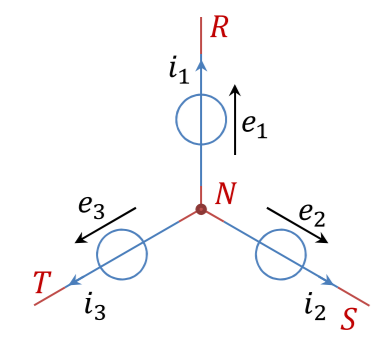
\includegraphics[width=5cm]{img/etoile.png}
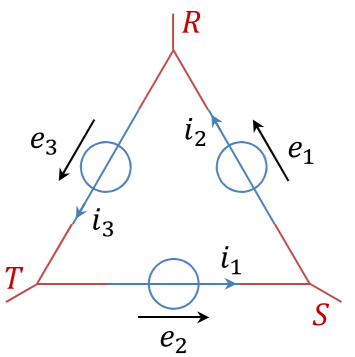
\includegraphics[width=5cm]{img/triangle.png}
\caption{à gauche: connection en étoile à droite: connection en triangle}
\end{figure}
On a l'apparition d'un point \textcolor{red}{neutre} $N$. Les tensions entre les points R,S et T sont les mêmes pour les deux formes.\\

Quand on y ajoute des charges, les tensions ne sont pas les mêmes pour les charges dans la formation triangles et étoiles.

\subsubsection{Intérêt}
\begin{figure}[H]
\centering
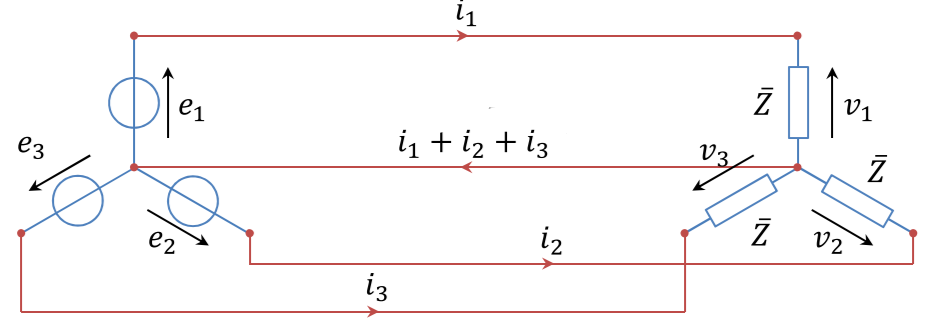
\includegraphics[width=10cm]{img/utilite.png}
\end{figure}
On peut supprimer le fil $i_1 + i_2 + i_3$ qui peut être supprimé car via les propriétés du \textit{triphasé} le courant s'annulent.

\subsection{Grandeurs de ligne}
Ce sont les grandeurs mesurées au niveau de la liaison source/charge:
\begin{itemize}
\item Courants de ligne: courants $i_R, i_S, i_T$ circulant dans les trois fils de liaison
\item Tensions de ligne: tensions $v_{RS}, v_{ST}, v_{TR}$ mesurées en prenant deux à deux les trois fils de liaison 
\end{itemize}

\subsection{Grandeurs de phase}
Ce sont les grandeurs mesurées sur les éléments qui constituent la source et/ou la charge:
\begin{itemize}
\item Courants de phase: courant $i_1, i_2, i_3$ circulant dans les sources ou les impédances constituant la source ou la charge triphasée.
\item Tensions de phase: tensions $v_1, v_2, v_3$ mesurées sur les sources ou les impédances constituant la source ou la charge triphasée.
\end{itemize}

\subsubsection{Cas particulier - étoile}
\begin{figure}[H]
\centering
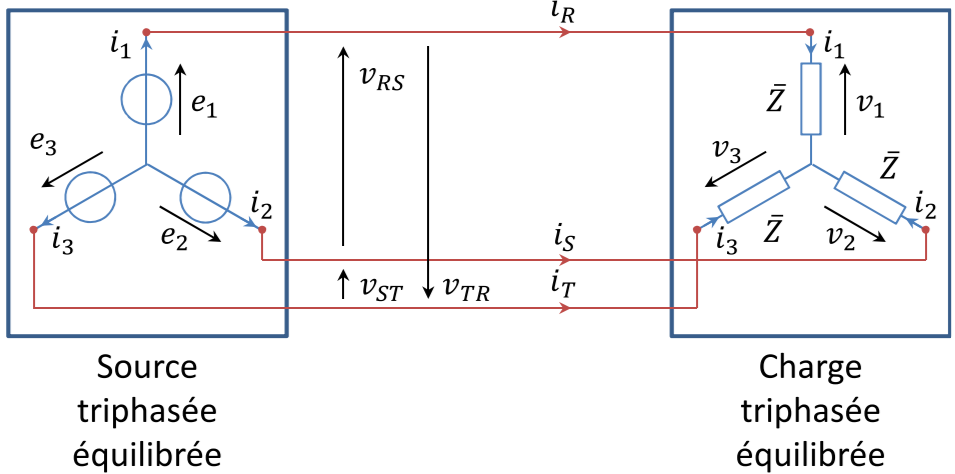
\includegraphics[width=8cm]{img/etoilesetoiles.png}
\end{figure}
Dans le cas ci-dessus, le courant de ligne et de phase est le même. La tension de ligne est tel que $V_l = \sqrt{3}V_{ph}$ et sa phase $\phi_l = \phi_{ph} + \frac{\pi}{6}$\par
Si on a une formation en \textit{triangle}, alors les courants de ligne et de phase sont différents entre eux.
\begin{align*}
V_l &= \sqrt{3} V_{ph} & \varphi_l &= \varphi_{ph} + \frac{\pi}{6} & I_l &= I_{ph} & \varphi_l &= \varphi_{ph}
\end{align*}

\subsubsection{Cas particulier - triangle}
Ressemble au cas en étoile mais cette fois-ci:
\begin{align*}
V_l &= V_{ph} & \varphi_l &= \varphi_{ph}& I_l &= \sqrt{3} I_{ph} & \varphi_l &= \varphi_{ph} + \frac{\pi}{6}
\end{align*}


\subsection{Circuit équivalent monophasé}
Puisque si nous possédons un circuit alimenté en \textbf{triphasé équilibré} en régime sinusoïdal, nous pouvons déterminé le courant et la tension dans toutes les broches si nous connaissons ceux-ci pour \textbf{une seule phase}.\par
Donc on peut étudier un tel circuit sur base de son équivalent \textbf{monophasé}.

\subsubsection{Mélange étoiles et triangles}
Selon les conventions, le circuit en \textcolor{red}{monophasé} est le circuit équivalent \textcolor{blue}{triphasé} obtenu en prenant \textit{une phase} du circuit triphasée et on remplace les \textbf{charges} et \textbf{sources} en leur \underline{équivalent étoile}.\par
L'avantage est que les grandeurs de phase et de ligne sont les mêmes.

\section{Transformation étoiles triangles}
On peut toujours passer de l'un à l'autre.
\begin{align*}
Z_{etoile} &= \frac{Z_{triangle}}{3} & V_{etoile} &= \frac{V_{triangle}}{\sqrt{3}} - \frac{\pi}{6}
\end{align*}
\begin{figure}[H]
\centering
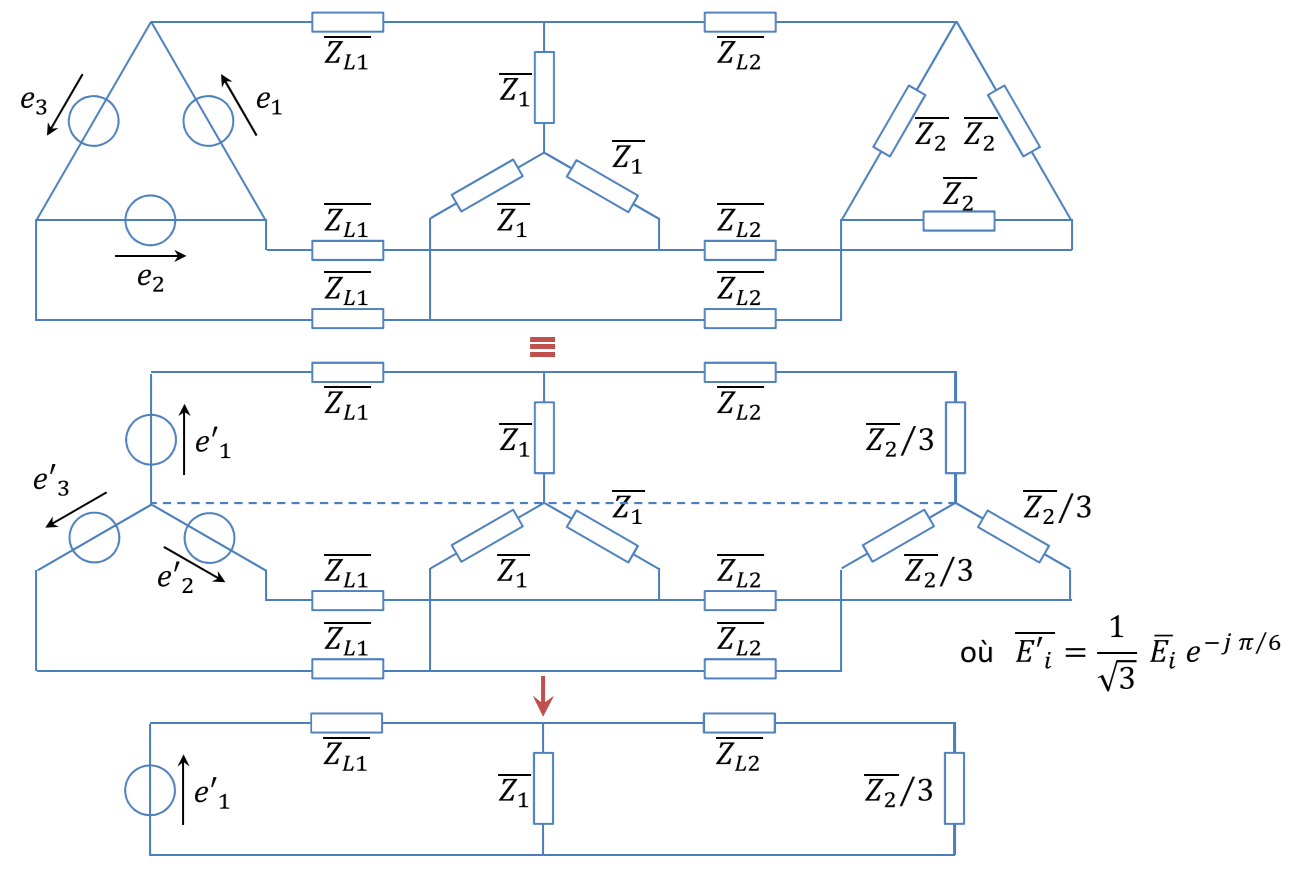
\includegraphics[width=12cm]{img/transfoEtoilesTriangles.png}
\caption{Transformation et équivalent monphasé}
\end{figure}

\subsection{Puissance}
\subsubsection{Puissance instantanée}
Pour un circuit équivalent monophasé:
\begin{align*}
p = ei &= P + S cos(2 \omega t + \varphi_v + \varphi_i) & &\begin{cases}
P = V_{eff}I_{eff} cos(\phi) = \frac{1}{2} V_{max} I_{max} cos(\phi) \text{     Puissance active}\\
S = V_{eff}I_{eff} = \frac{1}{2} V_{max} I_{max} \text{      Puissance apparente}
\end{cases}
\end{align*}
En triphasé:
\begin{equation}
p = e_1 i_1 + e_2 i_2 + e_3 i_3 = 3 V_{eff} I_{eff} cos(\phi) = \frac{3}{2} V_{max} I_{max} cos(\phi) = P
\end{equation}

\subsubsection{Puissance réactive}
\begin{equation}
Q = 3 V_{eff} I_{eff} sin(\phi)
\end{equation}

\subsubsection{Puissance apparente}
\begin{equation}
S = 3 V_{eff} I_{eff}
\end{equation}

\chapter{Circuits couplés magnétiquement}
\section{Introduction}
\subsection{Inductance}
\begin{wrapfigure}{r}{.4\textwidth}
\centering
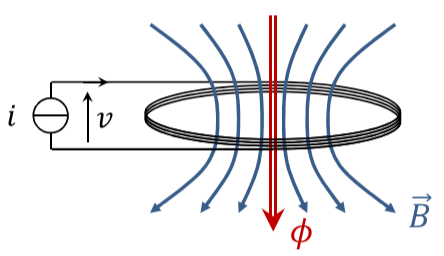
\includegraphics[width=5cm]{img/bobinage.png}
\end{wrapfigure}
Si on a un bobinage, comme ci-contre, qui est formé de $N$ spires et qu'on alimente d'une source de courant $i$. On génère ainsi un champ magnétique $\overrightarrow{B}$. Un certain flux $\phi$ traverse une spire. Ceci s'écrit $\phi = \int_S \overrightarrow{B} \overrightarrow{dS}$. Le flux $\Phi$ sur le \textit{bobinage} est $\Phi = N \phi$.\par
Si l'on considère le système sans \textbf{saturation magnétique}, on peut établir que $\Phi \propto i$. Ce facteur qui définit la \textcolor{red}{proportionnalité} est l'\textit{inductance} $L$. $\Phi = L i$.

\subsubsection{Loi de Faraday} 
La relation \textit{tension-courant} aux bornes du bobinage est donnée par la loi de \textbf{Faraday}:
\begin{align*}
v &= Ri + \frac{d\Phi}{dt} \text{ Loi de faraday} & e &= - \frac{d \Phi}{dt} \text{ Loi de Lenz}
\end{align*}
On peut négliger la \textit{résistance} et simplifier la relation à juste $v = L \frac{di}{dt}$.

\subsection{Inductances propre et mutuelle}
\begin{wrapfigure}{r}{.4\textwidth}
\centering
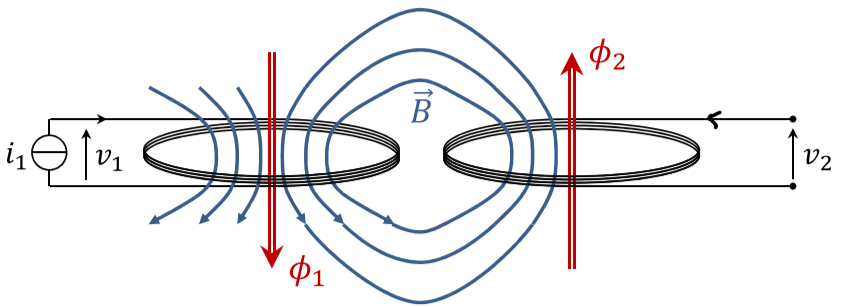
\includegraphics[width=6cm]{img/fluxMagnetique.png} 
\label{fig:mutuelle}
\end{wrapfigure}
Si nous avons $2$ bobinages, on peut faire apparaitre des courants \textit{induits}. On va voir apparaitre un courant et un champ magnétique opposé dans la deuxième partie. \par 
Ces deux champs et flux magnétiques vont essayer de se "\textit{tuer}". Cependant, les deux flux sont tels que $\Phi_1, \Phi_2 \propto i_1$.
\begin{align*}
\text{L'inductance propre: } L_1 &= \frac{\Phi_1}{i_1} & \text{L'inductance mutuelle: }  L_{21} &= \frac{\Phi_2}{i_1}\\
\text{Faraday : } v_1 &= L_1 \frac{di_1}{dt} & \text{Faraday : } v_2 &= L_{21} \frac{di_1}{dt}
\end{align*}

\subsubsection{Double alimentation}
Si maintenant, on alimente le circuit de droite et de gauche, on va obtenir un champ $\overrightarrow{B}$ qui est le résultat de deux champs créer par les deux circuits dépendant de l'inductance propre et mutuelle.\par
Ces facteurs de proportionnalité se définissent comme les inductances \textbf{propres} et \textbf{mutuelles}.
\begin{align*}
L_1 &=  \frac{\Phi_1}{i_1} \bigg|_{i_2 = 0} & L_{12} &=  \frac{\Phi_1}{i_2} \bigg|_{i_1 = 0} \\
L_2 &=  \frac{\Phi_2}{i_2} \bigg|_{i_1 = 0} & L_{21} &=  \frac{\Phi_2}{i_1} \bigg|_{i_2 = 0}
\end{align*}
On peut établir que $L_{12} = L_{21} = M$. Via loi de Faraday:
\begin{align*}
v_1 &= L_1 \frac{di_1}{dt} + M \frac{di_2}{dt} & v_2 &= M \frac{di_1}{dt} + L_2 \frac{di_2}{dt}
\end{align*}

Si nous inversons le courant dans l'un des circuits, on aura donc deux flux en \textit{parallèle}. Cela va créer une inversion de \textbf{norme} et donc rajouter des "$-$" devant les $M$.

\subsection{Bornes homologues}
On les repère par un \textit{point} au niveau d'une borne d'un bobinage. Quand on alimente ces bobinages par cette borne, on génère un flux de même sens dans les différents bobinages. On a donc des tensions positives.
\begin{figure}[H]
\centering
\includegraphics[width=7cm]{img/bornesHomologues.png}
\end{figure}
\subsubsection{En sinusoïdale}
Si on utilise des générateurs de courants/tensions sinusoïdaux, la définition devient:
\begin{align*}
\overline{V}_1 &= j \omega L_1 \overline{I}_1 + j \omega M \overline{I}_2 & \overline{V}_2 &= j \omega M \overline{I}_1 + j \omega L_2 \overline{I}_2
\end{align*}
La réactance est $X = \omega L$.

\section{Efficacité}
\subsection{Analyse énergétique}
On stocke l'énergie sous forme \textcolor{blue}{magnétique dans un bobinage}. Si on reprend le schéma \ref{fig:mutuelle}, on peut réaliser une analyse de l'énergie. On imagine que le bobinage de droite est en \textcolor{red}{circuit ouvert}.
\begin{align*}
E = \int_0^{t_1} (p_1(t) + p_2(t)) dt &= \int_0^{t1}v_1 (t) i_1 (t) dt\\
&= \int_0^{t_1} L_1 \frac{di_1 (t)}{dt} i_1 (t) dt\\
&= \int_0^{i_1 (t_1)} L_1 i_1(t) di_1(t)\\
E &= \frac{1}{2} L_1 I_1^2
\end{align*}
Si maintenant, on ferme le circuit à droite avec une source de courant $I_2$. On a maintenant une énergie:
\begin{align*}
E = \int_{t_1}^{t_2} (p_1(t) + p_2(t)) dt &= \int_{t_1}^{t_2} (v_1 (t) I_1 (t) + v_2(t) I_2 (t)) dt\\
&= \int_{t_1}^{t_2} \left( M \frac{di_1 (t)}{dt} + L_2 \frac{di_2 (t)}{dt} i_2 (t) \right) dt\\
&= \int_{0}^{i_2(t_2)} (M I_1 + L_2 i_2(t)) di_2(t)\\
E &= \frac{1}{2} L_2 I_2^2 + MI_1 I_1
\end{align*}
\textcolor{red}{Revoir les coefs au-dessus}
Ainsi, l'énergie magnétique totale stockée dans un tel système vaut:
\begin{equation}
E = \frac{1}{2} L_1 I_1^2 + \frac{1}{2} L_2 I_2^2 + MI_1 I_2
\end{equation}
Cette équation est valable uniquement si le courant est \textbf{entrant} ou \textbf{sortant} par les \textcolor{red}{bornes homologues} sinon:
\begin{equation}
E = \frac{1}{2} L_1 I_1^2 + \frac{1}{2} L_2 I_2^2 - MI_1 I_2
\end{equation}

\subsubsection{Analyse}
L'énergie dans le système \textbf{ne peut pas} être négative. Donc:
\begin{align*}
E &= \frac{1}{2} L_1 I_1^2 + \frac{1}{2} L_2 I_2^2 - M I_1 I_2 \geqslant 0 & L_1 L_2 &\geqslant M^2
\end{align*}

\subsection{Facteur de dispersion et coefficient de couplage}
\subsubsection{Cas idéal}
Il n'y a pas de flux de fuite et les flux sont \textit{intégralement} captés par les deux bobinages. On parle d'un \textbf{couplage magnétique parfait}.
\begin{equation}
M^2 = L_1 L_2
\end{equation}

\subsubsection{En réalité}
On a toujours un flux de fuite entre les deux bobinages donc $M \neq L_1 L_2$.
\begin{align*}
\text{Facteur de dispersion: } \sigma &= 1 - \frac{M^2}{L_1 L_2} & \text{Coefficient de couplage: } k &= \frac{M}{\sqrt{L_1 L_2}}
\end{align*}
Ici, $0 \leqslant \sigma \leqslant 1$ et $0 \leqslant k \leqslant 1$. Au plus $\sigma$ est faible au mieux c'est. Au plus $k$ est grand au mieux c'est.

\section{Transformateur idéal}
\begin{wrapfigure}{r}{.45\textwidth}
\centering
\includegraphics[width=6cm]{img/transfoBobinages.png}
\end{wrapfigure}
On couple deux bobinages à l'aide d'un entrefer pour ainsi rendre le transfert d'énergie optimale comme ci-contre.\par
On pose que la résistance électrique des bobinages null, pas de flux de fuite et perméabilité magnétique du circuit magnétique infinie. Via Faraday:
\begin{equation}
\frac{v_1}{v_2} = \frac{N_1}{N_2}
\end{equation}
On va maintenant réaliser la \textbf{loi d'Ampère} et on rajoute un parcours $\Gamma$ qui passe dans l'entrefer et les deux bobinages.
\begin{align*}
\int_{\Gamma} \overrightarrow{H} \overrightarrow{dl} &= N i & \int_{\Gamma} \overrightarrow{H} \overrightarrow{dl} &= N_1 i_1 + N_2 i_2\\
0 &= N_1 i_1 + N_2 i_2 & \frac{i_1}{i_2} &= - \frac{N_2}{N_1}
\end{align*}
On peut supposer que l'énergie est finie et donc que $N_1 i_1 + N_2 = 0$

\subsection{Analyse énergétique}
Donc on a que:
\begin{align*}
\frac{i_1}{i_2} &= - \frac{N_2}{N_1} &  \frac{v_1}{v_2} &=  \frac{N_1}{N_2} & \text{Puissance équivalente : } p_1 &= -p_2
\end{align*}
La puissance entrante est la même que la puissance sortante.

\subsection{Excitation sinusoïdale}
\begin{figure}[H]
\centering
\includegraphics[width=7cm]{img/transSinus.png}
\end{figure}
On peut ainsi travailler avec des \textit{phaseurs}. On indique le nombre de spire comme sur le schéma ci-dessus $N_1 : N_2$. Un transformateur idéal est indique via c'est barres en parallèle devant les bobinages. Relation tensions, courants:
\begin{align}
\frac{\overline{V_1}}{\overline{V_2}} &= \frac{1}{n} & \frac{\overline{I_1}}{\overline{I_2}} &= n & n &= \frac{N_2}{N_1}
\label{formulesSinus}
\end{align}

\subsubsection{Manipulation}
Quand on a ce type de circuit, on peut le transformer dans un modèle plus simple comme indiqué ci-dessous.
\begin{figure}[H]
\centering
\includegraphics[width=8cm]{img/manipTrans.png}
\end{figure}
On peut réaliser ce type de changement car on suppose le transfert d'énergie comme idéal.\par
La manipulation de ce type de circuit se repose sur l'utilisation des formules vu à l'équation \ref{formulesSinus}.


\chapter{Transformée de Laplace} \label{Laplace}
On va utiliser la transformée de Laplace \textit{bilatérale} qui n'est rien d'autre que la transformé de Fourier en complexe et qui est plus général.

\section{Équation différentielle avec Fourrier}
\begin{wrapfigure}{r}{.5\textwidth}
\centering
\begin{align*}
\frac{\partial^2 A(t)}{\partial t^2} + k^2 A(t) &= \delta (t)\\
A(\omega ) &= \frac{1}{k^2 - \omega^2}\\
A(t) &= \frac{1}{2\pi} \int_{-\infty}^{\infty} \frac{-e^{j \omega t}}{\omega^2 - k^2} d\omega \\
A(t) &= \frac{-2 \pi j}{2\pi} \left( \frac{e^{jkt}}{2k} - \frac{e^{-jkt}}{2k} \right)\\
A(t) &= \frac{sin(kt)}{k}
\end{align*}
\end{wrapfigure}
Si nous avons l'équation différentielle comme ci-contre, on va la transformer en équation dans le domaine \textbf{fréquentielle}.\par 
On passe d'une équation différentielle à une équation algébrique plus simple à résoudre. Sa solution en fréquentielle est $A(\omega)$. \par 
Donc on des \textit{pôles} en $\pm k$.\par 
On va appliquer le théorème des résidus pour intégrer sur $- \infty$ à $\infty$ en évitant les pôles. On fait une droite puis une demi arc de cercle.\par 
Une propriété extrêmement utile est \textcolor{red}{$df(t)/dt \rightarrow sF(s) -f(0)$}.\par 
Il faut aussi bien réduire en fraction simple.

\subsection{Résolution}
Les calculs sont longs et méthodiques, au début, il faut ré-écrire toutes les équations différentielles. Une fois qu'on a qu'une seule variable dans cette équation, on remplace les dérivées par leur équivalent en Fourier unilatéral. Si on a un signal qui passe de 2 à 1 Volts, il faut noter \textcolor{red}{$1 u(t)$} avec $u(t)$ la fonction échellon. Cela est important puisque qu'on passe d'une équation différentielle à une analyse en continue.

\chapter{Stabilité et systèmes}
On sait que la transformée de Laplace bilatérale est une transformée de Fourier pour $s = j \omega$ si la ROC contient $\sigma = 0$. On fait souvent référence à la transformée de Laplace unilatérale.

\section{Transformée inverse de Laplace}
On a une fonction $x(t) = e^{at} u(t)$ qui donne $X(s) = \frac{1}{s-a}$ sur $\mathfrak{R}(s) >a$. La transformée inverse est:
\begin{equation}
f(t) = \frac{1}{2 \pi j} \lim_{T\rightarrow \infty} \int_{k - j T}^{k + j T} F(s) e^{st} ds
\end{equation}

\subsection{Stabilité}
Un système est stable si \textbf{tous les pôles} de la fonction de \textcolor{red}{transfert} ont une partie réelle négative.
Ainsi, quand on repasse en temporel, nos exponentielles sont bornées et n'exploseront pas.

\section{Systèmes}
\subsection{Boucle fermée}
On va créer un chemin de retour pour minimiser l'erreur. Ainsi on peut comparer la valeur effective à la valeur recherchée. On a 3 types de régulateur:
\begin{enumerate}
\item \underline{P :} proportionnel donc simplement $H(s) = K_1$
\item \underline{PD :} proportionnel dérivé $H(s) = K_1 + K_3 s$
\item \underline{PID :} proportionnel intégrale dérivé $H(s) = K_1 + \frac{K_2}{s} + K_3 s$
\end{enumerate}
Les pôles en proportionnel dérivée sont tous sur l'axe des réelles et les PID sont en partie proche de l'origine.

\subsubsection{Soucis}
\begin{figure}[H]
\centering
\includegraphics[width=7cm]{img/regu.png}
\end{figure}
On peut voir sur le schéma:
\begin{itemize}
\item \underline{$y_0$ :} la réponse du système en boucle ouverte.
\item \underline{$y_p$ :} la réponse du système avec un régulateur de type proportionnel. On constate un overshoot très important et une convergence vers une valeur qui n’est pas la valeur désirée (avec une stabilisation très oscillatoire, qui n’est pas en soi problématique en elle-même mais l’overshoot l’est).
\item \underline{$y_{pd}$ :} la réponse du système avec un régulateur de type proportionnel dérivé. On constate un \textit{overshoot} pratiquement nul, une stabilisation rapide mais pas vers la bonne valeur.
\item \underline{$y_{pid}$ :} la réponse du système avec un régulateur de type proportionnel intégral dérivé. On constate qu’il n’y a pas d’overshoot, ça se stabilise très vite (plus vite que le système en boucle ouverte) vers la bonne valeur et c’est très stable. Un système PID est donc à
privilégier de manière générale
\end{itemize}

\subsection{Réponse à une harmonique infinie}
Très proche d'un phaseur quand on fait le calcul:
\begin{equation}
g(t) = \mathfrak{R}\{H(s = j \omega_o) e^{j \omega_o t}\}
\end{equation}

\subsection{Réponse à une harmonique causale}
Les pôles de la fonction de transfert sont responsable du transitoire et on a
\begin{equation}
g^h (t) = \mathfrak{R} \{H(s = j \omega_o) e^{j \omega_o t}\}
\end{equation}

\subsection{Décomposition en Harmonique}
On peut séparer notre fonction en série de sinus et cosinus (série de Fourier):
\begin{align*}
f_p (t) &= \sum_{n = - \infty}^{\infty} c_n e^{j n \omega_0 t} & c_n &= \frac{1}{T_0} \int_{- T_0 / 2}^{T_0 / 2} f(t) e^{-j n \omega_0 t} dt
\end{align*}
Ensuite, on peut voir le tout comme une sorte de convolution entre nos facteurs et un train de Dirac.


\chapter{Mesure}
\section{Erreurs et incertitudes}
\subsection{Erreurs vs. incertitudes}
\subsubsection{Erreur}
On nomme l'erreur comme $e$ qui est observé quand on mesure une valeur $x$ et son résultat réelle $\xi$.\\
L'erreur relative $e_r$ est le rapport entre l'erreur absolue $e$ et la valeur vraie $\xi$.\\ 
L'erreur $e$ peut avoir une composante \textbf{systématique} $\delta$ et une composante \textbf{aléatoire} $\epsilon$.
\begin{align} \label{eq:erreur}
e &\triangleq  x - \xi & e_r &\triangleq \frac{e}{\xi} & e &= \delta + \epsilon 
\end{align}

\subsubsection{Incertitudes}
C'est une \textit{estimation} de l'erreur \textbf{maximale} commise lors de la mesure. C'est donc un intervalle autour de la mesure avec une certaines probabilités où la valeur vraie se trouve. 


\subsection{Origine des erreurs}
Elles proviennent des instruments de mesures, de RLC cachés. Pour contrer les RLC cachés, on peut les inclure de manière explicite à notre circuit ou les annuler.\\
Le bruit électrique est aussi un facteur. On peut changer de composants qui génèrent moins de bruit. On peut aussi faire une moyenne sur différentes mesures.\\
L'interférence électrique est aussi un souci. On peut la diminuer via un blindage, filtrage ou un calcul des valeurs moyennes.\\
On observer aussi une variation de l'efficacité en fonction de la température des composants. Et certains composants peuvent différer des valeurs promises.
\subsubsection{Puissance prélevé par la mesure}
On va toujours essayer d'éviter les résistances en série. On probe toujours aux bornes de la résistances et non plus loin pour éviter de prendre en compte la résistivité des fils.

\subsubsection{Haute fréquence}
On utilise des câbles coaxiaux qui sont composés d'une âme qui n'est autre que le câble transportant le courant et d'une gaine. La gaine est une sorte de capacité mise en parallèle. Cela nous évite un pôle à $160 Hz$.\\

On utilise des câbles triaxiaux qui ont aussi une âme et une gaine mais possède une \textbf{garde} en plus. Cette garde est couplé à un suiveur pour obtenir un signal plus idéal.
\begin{figure}[H]
\centering
\includegraphics[width=8cm]{img/triaxial.png}
\caption{Représentation d'un câble triaxial}
\end{figure}

\subsection{Éléments de statistique}
Via nos équations précédentes (\ref{eq:erreur}) on peut établir que la valeur mesurée vaut $x = \xi + \delta + \epsilon$. Ceci suit une loi \textcolor{red}{normal} de $N(\mu , \sigma^2)$ où $\mu = \xi + \delta $.\par 
On dit qu'une mesure est reproductible si on a un écart type $\sigma$ faible donc un erreur aléatoire $\epsilon $ faible.\par 
La mesure exacte est la valeur moyenne $\mu$ proche de la valeur vraie $\xi$, donc une erreur systématique $\delta$ faible.

\subsubsection{Étalonnage}
On va essayer de supprimer l'erreur \textit{systématique} $\delta$. La valeur $2 \sigma$ correspond à l'incertitude absolue.


\subsection{Opérations arithmétiques sur les incertitudes}
Si on a deux mesures $A$ et $B$ qui n'ont aucune erreur systématique. De plus, $\epsilon_A$ et $\epsilon_B$ sont purement aléatoires et indépendantes.
\begin{equation}
\begin{cases}
x_A = \epsilon_A + \xi_A \quad \text{suivant la loi normal }N(0, \sigma_A^2)\\
x_B = \epsilon_B + \xi_B \quad \text{suivant la loi normal }N(0, \sigma_B^2)
\end{cases}
\end{equation}
La grandeur $Y = A \pm B$ à une caractéristique:
\begin{equation}
x_Y = \xi_A \pm \xi_B + \epsilon_Y \quad \text{suivant la loi normal }N(0, \sigma_Y^2)
\end{equation}
Et donc $\sigma_Y = \sqrt{\sigma_A^2 + \sigma_B^2}$.\\
La grandeur $Y = A * B$ à une caractéristique:
\begin{align*}
x_Y & \approx \xi_A * \xi_B * \left( 1 + \frac{\epsilon_A}{\xi_A} + \frac{\epsilon_B}{\xi_B}  \right) \\
& \approx \xi_A * \xi_B + \epsilon_Y \text{suivant la loi normal }N(0, \sigma_Y^2)\\
\sigma_Y &= \xi_A * \xi_B \sqrt{\left( \frac{\sigma_A}{\xi_A}\right)^2 + \left( \frac{\sigma_B}{\xi_B}\right)^2}
\end{align*}
La grandeur $Y = A / B$ à les caractéristiques suivantes:
\begin{align*}
x_Y &\approx \frac{\xi_A}{\xi_B} * \left( 1 + \frac{\epsilon_A}{\xi_A} - \frac{\epsilon_B}{\xi_B} \right)\\
& \approx \frac{\xi_A}{\xi_B} + \epsilon_Y  \text{suivant la loi normal }N(0, \sigma_Y^2)\\
\sigma_Y &= \frac{\xi_A}{\xi_B} \sqrt{\left( \frac{\sigma_A}{\xi_A}\right)^2 + \left( \frac{\sigma_B}{\xi_B}\right)^2}
\end{align*}

\section{Ponts pour la mesure d'impédance}
\subsection{Principe}
Les comparaisons sont beaucoup plus précises que des mesures absolues. Cela est utile pour les voltmètre numérique.

\subsection{Utilisation}
Mesure absolue de résistances par rapport à un standard. Cela est exacte à moins de $100$ ppm près. On peut mesurer de faible variations de résistance. On peut même mesurer des impédances.

\subsection{Pont de Wheatstone}
\begin{wrapfigure}{r}{.5\textwidth}
\centering
\includegraphics[width=7cm]{img/Wheatstone.png}
\end{wrapfigure}
On mesure des petite variations de résistances et on
 réalise des mesures absolues de résistance. On peut ainsi établir la fonction de transfert $H_W$:
\begin{align*}
H_W &= \frac{V_{AB}}{V_S} = \frac{R_{AY}}{R_{AX} + R_{AY}} - \frac{R_{BY}}{R_{BX} + R_{BY}}
\end{align*}
Ainsi, on peut réaliser 2 modes bien spécifiques, observer des faibles modifications:
\begin{align*}
R_{AX} &= (1 + \alpha) R\\
R_{AY} &= R_{BX} = R_{BY} = R\\
H_W &= \frac{\alpha}{2(2+\alpha)}
\end{align*}
Ou bien de faire des mesures absolues:
\begin{align*}
H_W &= V_{AB} = 0\\
R_{BX} &= R_{BY}\\
R_{AX} &= R_{AY}
\end{align*}

\subsection{Pont de Wien}
\begin{wrapfigure}{r}{.5\textwidth}
\centering
\includegraphics[width=7cm]{img/Wien.png}
\end{wrapfigure}
Ressemble très fort au pont de Wheatstone. Il faut bien remarquer le courant \textbf{AC} en entrée et pas DC. On a ces équations pour la fonction de transfert.
\begin{align*}
H_W &= \frac{V_{AB}}{V_S} = \frac{Z_{AY}}{Z_{AY} + Z_{AX}} - \frac{R_{BY}}{R_{BX} + R_{BY}}\\
& \begin{cases}
\frac{1}{Z_{AX}} = \frac{1}{R_{AX}} + j \omega_0 C_{AX}\\
Z_{AY} = R_{AY} - j \frac{1}{\omega_0 C_{AY}}
\end{cases}
\end{align*}
Pour mesurer, on veut que \textcolor{red}{$H_W = V_{AB} = 0$}:
\begin{align*}
\frac{Z_{AY}}{Z_{AX}} = \frac{R_{BY}}{R_{BX}} & \Longrightarrow \frac{R_{AY}}{R_{AX}} + \frac{C_{AX}}{C_{AY}} + j \left( \omega_0 R_{AY} C_{AX} - \frac{1}{\omega_0 R_{AX} C_{AY}} \right) = \frac{R_{BY}}{R_{BX}}\\
& \Longrightarrow \begin{cases}
R_{AX} = \frac{R_{BX}}{R_{BY}} \left( R_{AY} + \frac{1}{(\omega_0 C_{AY})^2 R_{AY}} \right)\\
C_{AX} = \frac{1}{\omega_0^2 C_{AY} R_{AY} R_{AX}}
\end{cases}
\end{align*}
\newpage

\subsection{Pont de Maxwell}
\begin{figure}[H]
\centering
\includegraphics[width=7cm]{img/Maxwell.png}
\end{figure}
Même idée que le pont de Wien mais pour les inductances, on va placer l'inductance sur l'autre coté.
\begin{align*}
H_W &= \frac{V_{AB}}{V_S} = \frac{Z_{AY}}{Z_{AY} + R_{AX}} - \frac{R_{BY}}{R_{BY} + Z_{BX}}\\
& \begin{cases}
Z_{BX} = R_{BX} + j \omega_0 L_{BX}\\
\frac{1}{Z_{AY}} = \frac{1}{R_{AY}} - j \omega_0 C_{AY}
\end{cases}
\end{align*}
Et pour mesurer l'inductance on veut que $H_W = V_{AB} = 0$ donc:
\begin{align*}
\frac{R_{AX}}{Z_{AY}} = \frac{Z_{BX}}{R_{BY}} & \Longrightarrow \frac{R_{AX}}{R_{AY}} + j \omega_0 R_{AX} C_{AY} = \frac{R_{BX}}{R_{BY}} + j \frac{\omega_0 L_{BX}}{R_{BY}}\\
& \Longrightarrow \begin{cases}
R_{BX} = R_{BY}\frac{R_{AX}}{R_{AY}}\\
L_{BX} = R_{BY}C_{AY}R_{AX}
\end{cases}
\end{align*}

\subsection{Impédances parasites en parallèle}
\begin{figure}[H]
\centering
\includegraphics[width=8cm]{img/Wagner.png}
\caption{Protection de Wagner}
\end{figure}
On fait face à un problème, on a un courant de fuite vers le blindage. On va donc annuler la tension aux bornes des éléments parasites les plus \textit{critiques}.\\
Ici, on annuler l'effet des courants de fuite des nœuds $A$ et $B$ vers la garde afin que l'équilibre soit \textit{correct}.

\end{document}


